\documentclass[11pt,a4paper]{article}
\usepackage[margin=26mm]{geometry}
\usepackage[T1]{fontenc}
\usepackage{lmodern,microtype}
\usepackage{amsmath,amssymb,amsthm,mathtools}
\usepackage{booktabs}
\usepackage{enumitem}
\usepackage{tikz}
\usetikzlibrary{arrows.meta,positioning,shapes.geometric,fit,calc}
\usepackage[colorlinks=true,linkcolor=blue!60!black,citecolor=green!40!black,urlcolor=blue!60!black]{hyperref}

\newtheorem{theorem}{Theorem}[section]
\newtheorem{lemma}[theorem]{Lemma}
\newtheorem{proposition}[theorem]{Proposition}
\newtheorem{corollary}[theorem]{Corollary}
\newtheorem{conjecture}[theorem]{Conjecture}
\newtheorem{imported}[theorem]{Imported theorem}
\newtheorem{mainthm}{Theorem}
\newtheorem{maincor}[mainthm]{Corollary}
\renewcommand{\themainthm}{\Alph{mainthm}}
\theoremstyle{definition}
\newtheorem{definition}[theorem]{Definition}
\newtheorem{remark}[theorem]{Remark}
\newtheorem{example}[theorem]{Example}

\emergencystretch=3em
\pdfstringdefDisableCommands{\def\alpha{alpha}\def\to{->}\def\infty{infinity}}
\newcommand{\E}{\mathbb{E}}
\newcommand{\PP}{\mathbb{P}}
\newcommand{\R}{\mathbb{R}}
\newcommand{\C}{\mathbb{C}}
\newcommand{\F}{\mathbb{F}}
\newcommand{\tr}{\operatorname{tr}}
\newcommand{\rank}{\operatorname{rank}}
\newcommand{\Cov}{\operatorname{Cov}}
\newcommand{\diag}{\operatorname{diag}}
\newcommand{\Gam}{\operatorname{Gamma}}
\newcommand{\Wish}{\operatorname{Wish}}
\newcommand{\tilt}{\mathrm{tilt}}
\newcommand{\vol}{\mathrm{vol}}
\newcommand{\RP}{\mathrm{RP}}

\title{Randomly pivoted Cholesky in a random frame\\ is dominated by volume sampling}
\author{}
\date{29 September 2026}

% Shared manuscript typography. Keep this file beside the manuscript folders.
\usepackage{needspace}
\usepackage{etoolbox}
\linespread{1.08}
\setlength{\parskip}{0.38em plus 0.08em minus 0.05em}
\setlength{\parindent}{1.25em}
\setlength{\emergencystretch}{2em}
\setlist{itemsep=4pt,topsep=6pt,parsep=2pt}
\renewcommand{\arraystretch}{1.16}
\setlength{\tabcolsep}{6pt}
\AtBeginDocument{%
  \setlength{\abovedisplayskip}{10pt plus 2pt minus 2pt}%
  \setlength{\belowdisplayskip}{10pt plus 2pt minus 2pt}%
  \setlength{\abovedisplayshortskip}{5pt plus 2pt}%
  \setlength{\belowdisplayshortskip}{8pt plus 2pt minus 2pt}%
}
\makeatletter
\def\th@plain{%
  \thm@preskip=10pt plus 2pt minus 2pt
  \thm@postskip=10pt plus 2pt minus 2pt
  \itshape
}
\def\th@definition{%
  \thm@preskip=10pt plus 2pt minus 2pt
  \thm@postskip=10pt plus 2pt minus 2pt
  \normalfont
}
\def\th@remark{%
  \thm@headfont{\itshape}%
  \thm@preskip=9pt plus 2pt minus 2pt
  \thm@postskip=9pt plus 2pt minus 2pt
  \normalfont
}
\makeatother
\AtBeginEnvironment{proof}{\Needspace{4\baselineskip}}
\widowpenalty=10000
\clubpenalty=10000
\displaywidowpenalty=10000
\raggedbottom

\begin{document}
\maketitle

\begin{abstract}
Can a random change of coordinates remove the worst cases of randomly pivoted Cholesky? We prove that for every real or complex positive semidefinite matrix $A$ and every pivot budget $k$, a single Haar rotation gives
\[
\E_{Q,\RP}\,\tr R_k(QAQ^*)\;\le\;(k+1)\,\frac{e_{k+1}(A)}{e_k(A)},
\]
where the right side is the expected trace error of volume sampling, interpreted as zero at and beyond rank exhaustion. Consequently, $r-1+\lceil r/\varepsilon\rceil$ pivots suffice for expected error $(1+\varepsilon)\tau_r(A)$. This is an average over the frame and the pivots. The proof identifies a spectral Markov chain and bounds its one-step expected ratio using a covariance inequality for independent Gamma variables. The comparison extends to every common Gamma shape and to energy-biased Gaussian probing. Colbrook's scale-separated example shows why the frame matters: in fixed coordinates the exact-budget ratio can approach $2^r$, whereas its Haar average is at most $r+1+o(1)$.
\end{abstract}

\tableofcontents
\clearpage
\section{Main results}\label{sec:main}

Randomly pivoted Cholesky chooses columns adaptively from the current residual. Its one-step mean trace decrease is determined by the spectrum, but its error after several steps can depend strongly on the eigenvectors. Our question is whether averaging over a random coordinate frame makes the complete process comparable to a spectral benchmark.

The answer is affirmative. Volume sampling provides the benchmark, and one initial Haar rotation is sufficient. The central result below holds for every positive semidefinite input, without a gap assumption, a decay condition, or a restriction on the pivot budget.

Throughout, $\F\in\{\R,\C\}$ and
\[
\alpha_\F=\tfrac12\ (\F=\R),\qquad \alpha_\F=1\ (\F=\C).
\]
For a positive semidefinite (PSD) matrix $B\in\F^{n\times n}$, one step of \emph{randomly pivoted Cholesky} (RP) selects an index $i$ with probability $B_{ii}/\tr B$ and replaces $B$ by the Schur complement
\[
B-\frac{Be_ie_i^*B}{B_{ii}},
\]
whose $i$-th row and column vanish. We write $R_k(B)$ for the residual after $k$ steps; once the residual is $0$ it stays $0$, so $R_k(B)=0$ for $k\ge\rank B$. For $|S|=k$ the residual after pivoting on $S$ is the Schur complement $A/A_{SS}$, which is the Nystr\"om residual $A-A_{:S}A_{SS}^{-1}A_{S:}$ \cite{CETW}.

Let $\lambda_1\ge\dots\ge\lambda_n\ge0$ be the eigenvalues of $A$, $e_j(A)=e_j(\lambda)$ the elementary symmetric polynomials, and $\tau_r(A)=\sum_{i>r}\lambda_i$. \emph{Volume sampling} (the $k$-DPP with kernel $A$) chooses $|S|=k$ with probability $\det A_{SS}/e_k(A)$; its expected residual trace is \cite{DRVW}
\begin{equation}\label{eq:Vk}
V_k(A):=\E_{\vol}\tr(A/A_{SS})=(k+1)\frac{e_{k+1}(A)}{e_k(A)},\qquad V_k(A):=0\ \text{ if } \rank A\le k.
\end{equation}
The convention in the second clause covers the case $e_k(A)=0$; when $\rank A=k$ the quotient is already $0$.

\begin{mainthm}[Random frames]\label{thm:A}
Let $A\in\F^{n\times n}$ be PSD and let $Q$ be Haar distributed on the orthogonal group $O(n)$ if $\F=\R$ and on the unitary group $U(n)$ if $\F=\C$, independent of the pivots. Then for every $k\ge0$,
\[
\E_{Q,\RP}\,\tr R_k(QAQ^*)\;\le\;V_k(A)=(k+1)\frac{e_{k+1}(A)}{e_k(A)}.
\]
Equality holds for $k\in\{0,1\}$ and for $k\ge\rank A$.
\end{mainthm}

\begin{maincor}[Pivot count]\label{cor:B}
For every $r\le k$, $V_k(A)\le\frac{k+1}{k+1-r}\,\tau_r(A)$. Hence, for every $\varepsilon>0$ and $r\ge1$,
\[
\E_{Q,\RP}\,\tr R_k(QAQ^*)\le(1+\varepsilon)\,\tau_r(A)\qquad\text{for } k=r-1+\lceil r/\varepsilon\rceil .
\]
\end{maincor}

The first inequality in Corollary~\ref{cor:B} is the volume-sampling bound of Guruswami and Sinop \cite{GS} (Imported Theorem~\ref{imp:GS}); with $k+1-r=\lceil r/\varepsilon\rceil$ the factor is $1+r/\lceil r/\varepsilon\rceil\le1+\varepsilon$.

\paragraph{Scope.} Theorem~\ref{thm:A} is an averaged statement about the expected trace of the \emph{rotated} algorithm. It is not stochastic domination of the error distribution, and by Markov's inequality it only gives $\PP_Q\{\E_{\RP}\tr R_k(QAQ^*)>cV_k(A)\}\le1/c$ over frames. It says nothing directly about RP in the given coordinates: Section~\ref{sec:contrast} gives inputs on which coordinate RP has $\E\tr R_r/\tau_r\to2^r$ at $k=r$, while the Haar average is at most $V_r\le(r+1)\tau_r$. Nor is the rotated scheme a column-selection method, so column-subset lower bounds do not speak to its optimality.

\subsection{The proof mechanism and its extensions}

The proof follows three reductions. First, the unused columns of a Haar basis remain conditionally Haar after an energy-biased pivot. Second, a Schur complement has an elementary-symmetric profile that is a mixture of eigenvalue deletions. Third, a covariance inequality controls the expected ratio of two such profiles. The following Gamma inequality supplies the final step.

\Needspace{9\baselineskip}
\begin{mainthm}[Lemma G]\label{thm:C}
Let $\alpha>0$, $c_1,\dots,c_d>0$, and let $y_i\sim\Gam(\alpha,\text{scale }c_i)$ be independent, $R=\sum_iy_i$. Let $u,v\in\R^d$. Suppose there is one ordering of $\{1,\dots,d\}$ along which $c$ is weakly monotone (in either direction), $u$ is weakly nondecreasing and $v$ is weakly nonincreasing. Then
\[
\E\Big[\frac{(y\cdot u)(y\cdot v)}{R}\Big]\;\E[R]\;\le\;\E[y\cdot u]\;\E[y\cdot v].
\]
\end{mainthm}

The rotated algorithm is the case $\alpha=\alpha_\F$ of a one-parameter family of Markov chains on spectra (Definition~\ref{def:alphachain}), in which each Schur step uses a direction whose squared coordinates in the current eigenbasis are $\mathrm{Dirichlet}(\alpha,\dots,\alpha)$.

\begin{mainthm}[The $\alpha$-family]\label{thm:D}
For every $\alpha\in(0,\infty)$, every PSD spectrum $\lambda$ and every $k$, the $\alpha$-chain started at $\lambda$ satisfies $\E^{(\alpha)}\tr_k\le V_k(\lambda)$. The two endpoints are exact:
\begin{enumerate}
\item[(i)] as $\alpha\to0$ the chain becomes successive (probability proportional to size) sampling of eigenvalues, i.e.\ coordinate RP on $\diag(\lambda)$, and the bound $\E_{\rm succ}\sum_{i\notin S}\lambda_i\le V_k(\lambda)$ persists;
\item[(ii)] at $\alpha=\infty$ the chain is deterministic and its trace after $k$ steps equals $V_k(\lambda)$ exactly.
\end{enumerate}
\end{mainthm}

\begin{mainthm}[Probing in tight frames; Gaussian probing]\label{thm:E}
Let $z_1,\dots,z_N\in\F^n$ and $q_i>0$ with $\sum_iq_iz_iz_i^*=I_n$. Energy-biased probing (select $z_i$ with probability $\propto q_i\,z_i^*Rz_i$, then update $R\leftarrow R-Rz_iz_i^*R/(z_i^*Rz_i)$) is exactly RP on the dilation $\widetilde A=D_q^{1/2}Z^*AZD_q^{1/2}$, whose residuals have the same nonzero spectra as those of the probing process. Moreover, energy-biased Gaussian probing (draw $w\sim N(0,I_n)$ over $\F$ with density tilted by $w^*Rw/\tr R$) has the same spectral law as RP in a Haar frame, so
\[
\E\,\tr R_k\le V_k(A)\le\frac{k+1}{k+1-r}\,\tau_r(A).
\]
\end{mainthm}

Plain Gaussian sketching, determinant-tilted Gaussian sketching and energy-biased Gaussian probing are the Gaussian-dilation analogues of uniform sampling, volume sampling and RP; their constants are $1+\frac{r}{m-r-1}$, $\frac{m+1}{m-r+1}$, and (by Theorem~\ref{thm:E}) again at most $\frac{m+1}{m-r+1}$ (Section~\ref{sec:dilation}).

\begin{mainthm}[Gaussian-row population chain]\label{thm:F}
Let $C$ be an $r\times r$ PSD prior, and run the chain $V_0=C$,
\[
V_{s+1}=V_s-\frac{V_sz z^*V_s}{1+z^*V_sz},\qquad z\sim N(0,I_r)\ \text{over }\F\ \text{tilted by}\ \frac{1+z^*V_sz}{1+\tr V_s}.
\]
Then $\E\tr V_k\le(k+1)E_{k+1}(C)/E_k(C)-1$ with $E_m(C)=\sum_{j}e_j(C)/(m-j)!$; in particular $\E\tr V_k\le r/(k+1-r)$ for every $k\ge r$ and every prior.
\end{mainthm}

Theorem~\ref{thm:F} is unconditional. It follows from Theorem~\ref{thm:E} applied to the inputs $\diag(C,N^{-1}I_N)$ and a fixed-$k$ limit lemma (Lemma~\ref{lem:weak}), which we prove by coupling all $N$ on one probability space and applying Fatou's lemma.

\subsection{Relation to earlier work and the contribution}

Chen, Epperly, Tropp and Webber \cite{CETW} developed the modern low-rank analysis of RPCholesky and documented earlier appearances of the pivot rule. We use their residual formulation and the familiar conditional trace identity. Epperly \cite[Cor.~1.3]{Epperly2026} improves the coordinate pivot-count analysis to $r/\varepsilon+2r\sqrt{\log r}+r\log(1/\varepsilon)+2.3r$; Divan and Gilles \cite{DG} study spectral-decay rates and approximate pivot distributions. These results concern the given coordinates, while our comparison concerns a changed algorithmic input.

Volume sampling for low-rank approximation was developed by Deshpande, Rademacher, Vempala and Wang \cite{DRVW}, with adaptive sampling studied in \cite{DV}. Its elementary-symmetric benchmark and the factor $(k+1)/(k+1-r)$ of Guruswami and Sinop \cite{GS} are prior results. Determinantal sampling and regression applications are discussed in \cite{BW,KT,DW,DWH}.

The diagonal endpoint also has prior substance. There, RP is successive sampling, and volume sampling is rejective sampling. Yu \cite{Yu} proved the relevant ordering of inclusion probabilities, resolving a question of H\'ajek \cite{Hajek}. Our endpoint argument recovers the weighted residual comparison; we do not claim that comparison as new.

The contribution of this paper is the comparison for a \emph{single Haar-rotated arbitrary PSD matrix}, including both real and complex frames. It rests on the spectral reduction and the Gamma covariance argument, rather than on the diagonal inclusion-probability theorem. The Gaussian-probing comparison and the prior-uniform population bound are consequences of that argument. The scale-separated example in Section~\ref{sec:contrast} is explicitly attributed to Colbrook's construction. The inverse-Wishart calculation uses classical Schur-complement and Bartlett identities and is presented as a useful specialization of those facts. The novelty claimed here is the Haar comparison and its Gamma-chain proof; it does not include the volume benchmark, the diagonal endpoint, or the classical Wishart identities.

\begin{figure}[t]
\centering
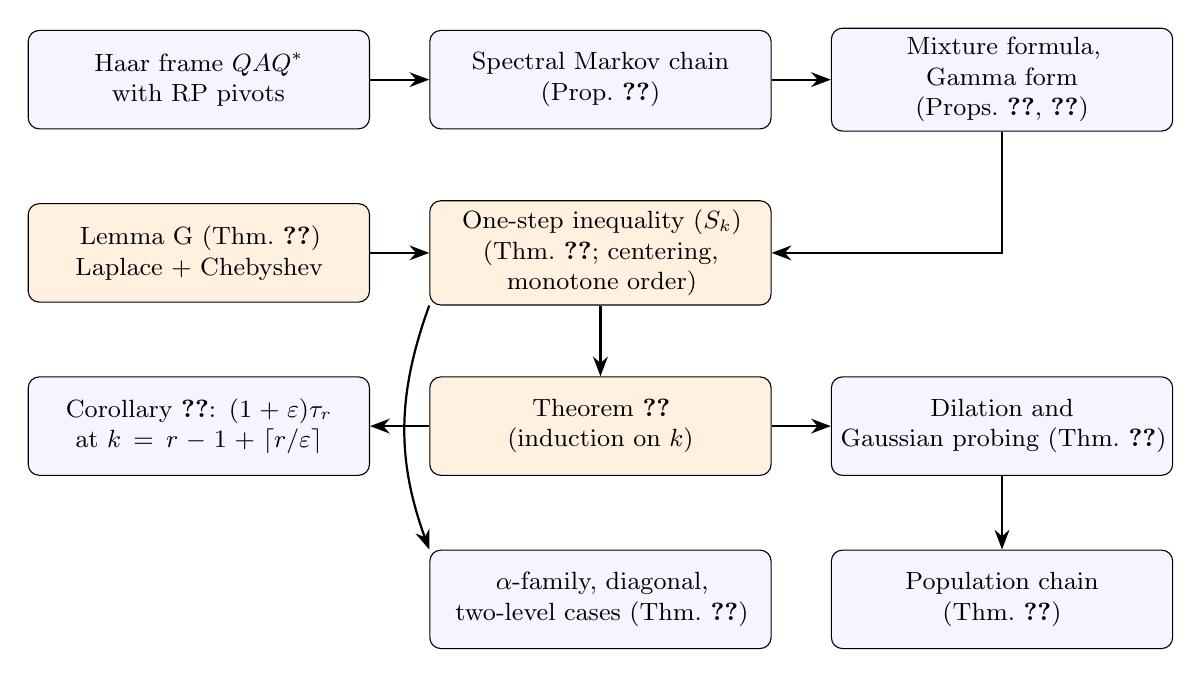
\begin{tikzpicture}[
  box/.style={draw,rounded corners,align=center,font=\small,minimum height=1.25cm,text width=4.1cm,fill=blue!4},
  key/.style={box,fill=orange!12},
  arr/.style={-{Stealth[length=2.5mm]},thick}]
\node[box] (frame) at (0,0) {Haar frame $QAQ^*$\\ with RP pivots};
\node[box] (chain) at (5.1,0) {Spectral Markov chain\\ (Prop.~\ref{prop:markov})};
\node[box] (mix) at (10.2,0) {Mixture formula, Gamma form\\ (Props.~\ref{prop:mixture}, \ref{prop:gamma})};
\node[key] (G) at (0,-2.2) {Lemma G (Thm.~\ref{thm:C})\\ Laplace + Chebyshev};
\node[key] (Sk) at (5.1,-2.2) {One-step inequality $(S_k)$\\ (Thm.~\ref{thm:Sk}; centering,\\ monotone order)};
\node[key] (A) at (5.1,-4.4) {Theorem~\ref{thm:A}\\ (induction on $k$)};
\node[box] (cor) at (0,-4.4) {Corollary~\ref{cor:B}: $(1+\varepsilon)\tau_r$\\ at $k=r-1+\lceil r/\varepsilon\rceil$};
\node[box] (E) at (10.2,-4.4) {Dilation and\\ Gaussian probing (Thm.~\ref{thm:E})};
\node[box] (Dfam) at (5.1,-6.6) {$\alpha$-family, diagonal,\\ two-level cases (Thm.~\ref{thm:D})};
\node[box] (F) at (10.2,-6.6) {Population chain\\ (Thm.~\ref{thm:F})};
\draw[arr] (frame)--(chain); \draw[arr] (chain)--(mix);
\draw[arr] (mix.south) |- (Sk.east); \draw[arr] (G)--(Sk);
\draw[arr] (Sk)--(A); \draw[arr] (A)--(cor); \draw[arr] (A)--(E); \draw[arr] (E)--(F);
\draw[arr] (Sk.south west) to[bend right=20] (Dfam.north west);
\end{tikzpicture}
\caption{Roadmap of the proof. Orange boxes carry the inequality content; the other boxes are exact identities or reductions.}
\label{fig:roadmap}
\end{figure}

\paragraph{Organization.} Section~\ref{sec:prelim} collects identities. Section~\ref{sec:reduction} reduces Theorem~\ref{thm:A} to the one-step inequality. Section~\ref{sec:lemmaG} proves Lemma~G, and Section~\ref{sec:proof} completes the proof. Section~\ref{sec:family} treats the $\alpha$-family and the special cases, Section~\ref{sec:contrast} the coordinate contrast, Section~\ref{sec:dilation} tight frames and Gaussian probing, and Section~\ref{sec:population} the population chain and the Wishart identity. Numerical evidence is in Section~\ref{sec:numerics}, the interpretation in Section~\ref{sec:meaning}, and open problems in Section~\ref{sec:open}.
\section{Preliminaries}\label{sec:prelim}

\subsection{Elementary symmetric polynomials}
For a finite list $\Lambda=(\lambda_1,\dots,\lambda_d)$ of nonnegative reals write $e_j(\Lambda)$ for its elementary symmetric polynomials ($e_0=1$, $e_j=0$ for $j<0$ or $j>d$), $\Lambda_{-i}$ for the list with $\lambda_i$ removed, and $\Lambda_{-ij}$ for the list with $\lambda_i,\lambda_j$ removed. We use three identities, each immediate from the generating function $\prod_i(1+t\lambda_i)=\sum_je_jt^j$:
\begin{align}
e_j(\Lambda)&=e_j(\Lambda_{-i})+\lambda_ie_{j-1}(\Lambda_{-i}),\label{eq:e-split}\\
\sum_i\lambda_i\,e_j(\Lambda_{-i})&=(j+1)\,e_{j+1}(\Lambda),\label{eq:e-euler}\\
\det(xI+\diag\Lambda)&=\sum_{j}e_j(\Lambda)\,x^{d-j}.\label{eq:e-charpoly}
\end{align}
Identity \eqref{eq:e-euler} counts each $(j+1)$-subset once for each of its elements.

\begin{imported}[Newton's inequality {\cite[Thm.~51]{HLP}}]\label{imp:newton}
For nonnegative reals and every $m\ge1$, $e_m(\Lambda)^2\ge e_{m-1}(\Lambda)\,e_{m+1}(\Lambda)$.
\end{imported}
The classical statement is for the normalized means $e_m/\binom dm$; the unnormalized form follows because $\binom dm^2\ge\binom d{m-1}\binom d{m+1}$.

\subsection{Chebyshev's sum inequality with weights}
Let $\pi$ be a probability vector on $\{1,\dots,d\}$ and $a,b\in\R^d$. Then
\begin{equation}\label{eq:cheb}
\Cov_\pi(a,b)=\tfrac12\sum_{i,j}\pi_i\pi_j(a_i-a_j)(b_i-b_j).
\end{equation}
Call $a$ and $b$ \emph{similarly ordered} if there is one ordering of the indices along which both are weakly nondecreasing, and \emph{oppositely ordered} if along one ordering $a$ is weakly nondecreasing and $b$ weakly nonincreasing. By \eqref{eq:cheb}, $\Cov_\pi(a,b)\ge0$ for similarly ordered and $\Cov_\pi(a,b)\le0$ for oppositely ordered vectors, for \emph{every} probability vector $\pi$. We use this repeatedly, always with one fixed ordering, so that all vectors involved are compared along the same order.

\subsection{Volume sampling}
\begin{imported}[Expected residual of volume sampling {\cite{DRVW}}]\label{imp:DRVW}
If $S$ is drawn with probability $\det A_{SS}/e_k(A)$ among $k$-subsets, then $\E\tr(A/A_{SS})=(k+1)e_{k+1}(A)/e_k(A)$. More generally $\E\,e_\ell(A/A_{SS})=\binom{k+\ell}{\ell}e_{k+\ell}(A)/e_k(A)$.
\end{imported}
The general form follows from the determinant identity
\[
\det A_{SS}\,e_\ell(A/A_{SS})=\sum_{T\supset S,\,|T|=k+\ell}\det A_{TT},
\]
summed over $S$; it is also a special case of Proposition~\ref{prop:volrescaled} below.

\begin{imported}[Guruswami--Sinop {\cite{GS}}]\label{imp:GS}
For every PSD $A$ and $r\le k$, $(k+1)\,e_{k+1}(A)/e_k(A)\le\frac{k+1}{k+1-r}\,\tau_r(A)$.
\end{imported}

\begin{proof}
Every $(k+1)$-subset contains at least $k+1-r$ indices beyond the first $r$. Counting those indices in the products defining $e_{k+1}$ gives
\begin{align*}
(k+1-r)e_{k+1}(A)
&\le \sum_{i>r}\lambda_i e_k(\Lambda_{-i})\\
&\le \tau_r(A)e_k(A).
\end{align*}
Divide by $e_k(A)>0$ and multiply by $k+1$. Rank exhaustion is covered by the zero convention. This elementary proof records the particular consequence of \cite{GS} used here.
\end{proof}

\subsection{Gamma and Dirichlet variables}
Write $\Gam(\alpha,\text{scale }c)$ for the law with density $x^{\alpha-1}e^{-x/c}/(\Gamma(\alpha)c^\alpha)$ on $(0,\infty)$. We use:
\begin{enumerate}
\item[(G1)] If $u$ is uniform on the unit sphere of $\F^d$ and $g_1,\dots,g_d$ are i.i.d.\ $\Gam(\alpha_\F,1)$ with $G=\sum_ig_i$, then $(|u_1|^2,\dots,|u_d|^2)$ has the law of $g/G$ (a $\mathrm{Dirichlet}(\alpha_\F,\dots,\alpha_\F)$ vector), and $G$ is independent of $g/G$ (Lukacs). Indeed $u=\gamma/|\gamma|$ for a standard Gaussian vector $\gamma$ over $\F$, and $|\gamma_i|^2$ is $\Gam(\frac12,\text{scale }2)$ for $\F=\R$ and $\Gam(1,1)$ for $\F=\C$ (with $\E|\gamma_i|^2=1$); a common scale factor cancels in $g/G$.
\item[(G2)] For $y\sim\Gam(\alpha,\text{scale }c)$ and $t\ge0$,
\[
\E e^{-ty}=(1+tc)^{-\alpha},\quad \E\,ye^{-ty}=\alpha c(1+tc)^{-\alpha-1},\quad \E\,y^2e^{-ty}=\alpha(\alpha+1)c^2(1+tc)^{-\alpha-2}.
\]
\end{enumerate}

\subsection{Conventions at rank exhaustion}\label{sec:conventions}
For a PSD operator $M$ on a finite-dimensional space, $V_j(M)=(j+1)e_{j+1}(M)/e_j(M)$ if $\rank M>j$ and $V_j(M)=0$ if $\rank M\le j$. If $\rank M=j$ the quotient formula also gives $0$, so the two clauses agree there. A Schur step $M\mapsto M-Muu^*M/(u^*Mu)$ with $u^*Mu>0$ lowers the rank by exactly one: writing $P$ for the orthogonal projection onto the nonzero vector $M^{1/2}u$, the updated operator is $M^{1/2}(I-P)M^{1/2}$, whose rank is $\rank\big((I-P)M^{1/2}\big)=\rank M^{1/2}-1$ because $M^{1/2}u\in\operatorname{im}M^{1/2}$. All processes below stop once the residual is $0$; the residual trace is then $0$ at all later times.
\section{Reduction to a spectral Markov chain}\label{sec:reduction}

\subsection{The frame chain}
Let $W\subseteq\F^n$ be a subspace and $M$ a PSD operator on $W$. For a unit vector $u\in W$ with $u^*Mu>0$ put
\[
M_u:=M-\frac{Muu^*M}{u^*Mu}.
\]
$M_u$ is PSD, self-adjoint on $W$, and $M_uu=0$; hence it maps $W\cap u^\perp$ into itself, and we regard it as an operator there. Let $\sigma_W$ be the uniform probability measure on the unit sphere of $W$, and let the \emph{energy-tilted} law be
\begin{equation}\label{eq:tilt}
\tilt_M(du)=\frac{u^*Mu}{\E_{\sigma_W}[u^*Mu]}\,\sigma_W(du)=\frac{\dim W}{\tr M}\,u^*Mu\;\sigma_W(du).
\end{equation}

\begin{definition}[Frame chain]\label{def:framechain}
Start from $(W_0,M_0)=(\F^n,A)$. Given $(W_s,M_s)$ with $M_s\ne0$, draw $u_{s+1}\sim\tilt_{M_s}$ and set $W_{s+1}=W_s\cap u_{s+1}^\perp$, $M_{s+1}=(M_s)_{u_{s+1}}$. If $M_s=0$ the chain stops, and $M_t=0$ for $t\ge s$.
\end{definition}

\begin{proposition}[Markov reduction]\label{prop:markov}
Let $Q$ be Haar on $O(n)$ or $U(n)$ and run RP on $B=QAQ^*$. Then the process $(\tr R_s(B))_{s\ge0}$ has the same law as $(\tr M_s)_{s\ge0}$ for the frame chain started at $(\F^n,A)$.
\end{proposition}

\begin{proof}
Put $q_i=Q^*e_i$. Since $Q^*$ is Haar, $(q_1,\dots,q_n)$ is a Haar-random orthonormal basis of $\F^n$, and $B_{ij}=q_i^*Aq_j$. We show by induction on $s$ the following statement. Condition on the first $s$ pivots $i_1,\dots,i_s$ and on the vectors $q_{i_1},\dots,q_{i_s}$. Then the remaining vectors $(q_j)_{j\notin S_s}$ form a Haar-random orthonormal basis of $W_s=\operatorname{span}(q_{i_1},\dots,q_{i_s})^\perp$. Moreover $R_s(B)_{jl}=q_j^*M_sq_l$ for $j,l\notin S_s$, the rows and columns indexed by $S_s$ vanish, and $M_s$ is the operator obtained from $A$ by the successive updates along $q_{i_1},\dots,q_{i_s}$.

For $s=0$ this is the definition. Suppose it holds at $s$ and $M_s\ne0$. Since $(q_j)_{j\notin S_s}$ is an orthonormal basis of $W_s$, $\tr R_s(B)=\tr M_s$. RP picks $j\notin S_s$ with probability $q_j^*M_sq_j/\tr M_s$. Under the Haar law each $q_j$ is uniform on the unit sphere of $W_s$, and given $q_j$ the other basis vectors are Haar on $W_s\cap q_j^\perp$. The selection weight depends on the basis only through $q_j$, and its normalizer $\tr M_s$ does not depend on the basis at all. Hence, conditionally on the event that $j$ is picked, $q_j$ has the law $\tilt_{M_s}$ (the same for every $j$), and given $q_j$ the remaining vectors are still Haar on $W_s\cap q_j^\perp=W_{s+1}$. Finally
\[
R_{s+1}(B)_{ab}=q_a^*M_sq_b-\frac{(q_a^*M_sq_j)(q_j^*M_sq_b)}{q_j^*M_sq_j}=q_a^*(M_s)_{q_j}q_b .
\]
This completes the induction. The index $j$ carries no information about the future traces, so the pivot directions $q_{i_1},q_{i_2},\dots$ have the law of the chain directions $u_1,u_2,\dots$, and $\tr R_s(B)=\tr M_s$ for all $s$.
\end{proof}

A single initial rotation suffices; the algorithm is not re-rotated between steps. The conditional Haar invariance of the unused basis vectors is the only property of the Haar measure that is used.

\subsection{The mixture formula}
\begin{proposition}[Mixture formula]\label{prop:mixture}
Let $M$ be PSD on $W$ ($\dim W=m$) with eigenvalues $\lambda_1,\dots,\lambda_m$ and orthonormal eigenvectors $v_1,\dots,v_m$, and let $u\in W$ be a unit vector with $u^*Mu>0$. Put $u_i=v_i^*u$ and $w_i=\lambda_i|u_i|^2/\sum_j\lambda_j|u_j|^2$. Then
\begin{equation}\label{eq:mixture}
\begin{aligned}
\det(xI_W+M_u)&=\sum_{i=1}^mw_i\,x\prod_{j\ne i}(x+\lambda_j),\\
e_\ell(M_u)&=\sum_iw_i\,e_\ell(\Lambda_{-i})\qquad(\ell\ge0).
\end{aligned}
\end{equation}
Under $u\sim\tilt_M$ one has $\E_\tilt w_i=\lambda_i/\tr M$ and
\begin{equation}\label{eq:Eel}
\E_\tilt e_\ell(M_u)=\frac{(\ell+1)\,e_{\ell+1}(M)}{\tr M}.
\end{equation}
\end{proposition}

\begin{proof}
Let $\mu=u^*Mu$ and $x>0$. By the matrix determinant lemma,
\begin{align*}
\det(xI+M_u)
&=\det(xI+M)\left(1-\frac{u^*M(xI+M)^{-1}Mu}{\mu}\right)\\
&=\frac{\det(xI+M)}{\mu}
  \sum_i\lambda_i|u_i|^2\left(1-\frac{\lambda_i}{x+\lambda_i}\right).
\end{align*}
and $1-\lambda_i/(x+\lambda_i)=x/(x+\lambda_i)$. Multiplying out gives \eqref{eq:mixture} for $x>0$, hence as a polynomial identity. Comparing coefficients with \eqref{eq:e-charpoly}, using $x\prod_{j\ne i}(x+\lambda_j)=\sum_\ell e_\ell(\Lambda_{-i})x^{m-\ell}$, gives the second formula. For the expectations, $\E_{\sigma_W}|u_i|^2=1/m$, so by \eqref{eq:tilt} $\E_\tilt w_i=\frac m{\tr M}\E_{\sigma_W}[\lambda_i|u_i|^2]=\lambda_i/\tr M$. Then \eqref{eq:Eel} follows from \eqref{eq:e-euler}.
\end{proof}

For $\ell=1$, \eqref{eq:Eel} gives
\[
\E_\tilt\tr M_u=\frac{2e_2(M)}{e_1(M)}=V_1(M).
\]
The same first-step mean holds in any fixed orthonormal frame, because energy weighting cancels the Schur denominator. The difficulty begins at the second step: the residual spectrum is random, so one must control an expected ratio. In fact, \eqref{eq:e-euler} rewrites the target as
\[
V_k(M)=k\,\frac{\E_\tilt e_k(M_u)}{\E_\tilt e_{k-1}(M_u)}.
\]

\subsection{Gamma form of the tilted law}
\begin{proposition}[Gamma form]\label{prop:gamma}
In the setting of Proposition~\ref{prop:mixture}, let $g_1,\dots,g_m$ be i.i.d.\ $\Gam(\alpha_\F,1)$ and $S=\sum_i\lambda_ig_i$. If $F:[0,\infty)^m\to[0,\infty]$ is measurable and $0$-homogeneous, $F(tg)=F(g)$ for $t>0$, then
\[
\E_{u\sim\tilt_M}F\big(|u_1|^2,\dots,|u_m|^2\big)=\frac{\E[S\,F(g)]}{\E[S]},\qquad \E[S]=\alpha_\F\tr M.
\]
The same holds for bounded signed $F$.
\end{proposition}

\begin{proof}
Write $G=\sum_ig_i$. By (G1), $(|u_i|^2)_i\sim g/G$ and $u^*Mu\sim S/G$, and $G$ is independent of $g/G$. Since $S/G$ and $F(g)=F(g/G)$ are functions of $g/G$,
\[
\E[S\,F(g)]=\E\big[G\cdot(S/G)F(g/G)\big]=\E[G]\;\E_{\sigma_W}[(u^*Mu)F],
\]
and likewise $\E[S]=\E[G]\,\E_{\sigma_W}[u^*Mu]$. Divide and use \eqref{eq:tilt}.
\end{proof}

Note that $G$ runs over all $m$ coordinates, including those of zero eigenvalues; these coordinates enter neither $S$ nor the weights $w_i$, which are $0$-homogeneous in $g$.

\subsection{The $\alpha$-chain and the induction}
Proposition~\ref{prop:mixture} shows that the spectrum of $M_u$ is a function of $\lambda$ and the weights $w$, and Proposition~\ref{prop:gamma} gives the law of $w$. This defines a chain on spectra for every Gamma shape.

\begin{definition}[$\alpha$-chain]\label{def:alphachain}
Let $\alpha>0$. The state is the list $\Lambda=(\lambda_1,\dots,\lambda_d)$ of positive eigenvalues; the empty list is absorbing. Given $\Lambda$, draw $g_1,\dots,g_d$ i.i.d.\ $\Gam(\alpha,1)$ under the tilted law $\frac{S}{\E S}\,d\PP$ with $S=\sum_i\lambda_ig_i$, put $w_i=\lambda_ig_i/S$, and let the next state be the positive roots, negated, of
\[
p(x)=\sum_{i=1}^dw_i\prod_{j\ne i}(x+\lambda_j).
\]
We write $\E_\tilt$ for expectation over one step, $\tr_s$ for the sum of the state after $s$ steps, and $F^{(\alpha)}_k(\Lambda)=\E\tr_k$ for the chain started at $\Lambda$.
\end{definition}

The polynomial $p$ has $d-1$ nonpositive real roots: realizing $M=\diag\Lambda$ and $u_i=\sqrt{g_i/G}$, Proposition~\ref{prop:mixture} gives $x\,p(x)=\det(xI+M_u)$ with $M_u$ PSD of rank $d-1$. So the state loses exactly one positive eigenvalue per step and is empty after $d$ steps. By Propositions~\ref{prop:markov}--\ref{prop:gamma} and \eqref{eq:mixture}:

\begin{corollary}\label{cor:chainid}
For PSD $A$ over $\F$, $\E_{Q,\RP}\tr R_k(QAQ^*)=F_k^{(\alpha_\F)}(\lambda(A))$ for every $k$.
\end{corollary}

For $\Lambda$ with at least $k$ positive entries, the one-step inequality at budget $k\ge2$ is
\[
(S_k^{(\alpha)})\qquad\E_\tilt V_{k-1}(\Lambda')\le V_k(\Lambda),
\]
where $\Lambda'$ is the next state of the $\alpha$-chain.

\begin{proposition}[Induction]\label{prop:induction}
Fix $\alpha>0$. If $(S_k^{(\alpha)})$ holds for all $k\ge2$ and all spectra with at least $k$ positive entries, then $F^{(\alpha)}_k(\Lambda)\le V_k(\Lambda)$ for all $k\ge0$ and all $\Lambda$, with equality for $k\in\{0,1\}$ and for $k\ge|\Lambda|$.
\end{proposition}

\begin{proof}
$F_0=e_1=V_0$. For $k=1$ and $\Lambda\neq\emptyset$, $F_1(\Lambda)=\E_\tilt e_1(\Lambda')=2e_2(\Lambda)/e_1(\Lambda)=V_1(\Lambda)$ by \eqref{eq:Eel}; this is an identity, not an inequality. If $|\Lambda|\le k$, the state is empty after $|\Lambda|$ steps, so $F_k(\Lambda)=0=V_k(\Lambda)$ by the conventions of Section~\ref{sec:conventions}. Let $k\ge2$, $|\Lambda|\ge k+1$, and assume $F_{k-1}\le V_{k-1}$ on all spectra. By the Markov property,
\[
F_k(\Lambda)=\E_\tilt F_{k-1}(\Lambda')\le\E_\tilt V_{k-1}(\Lambda')\le V_k(\Lambda),
\]
where $|\Lambda'|=|\Lambda|-1\ge k$ almost surely, so $e_{k-1}(\Lambda')>0$ and no $0/0$ occurs.
\end{proof}

\begin{remark}[Budget two is decisive]\label{rem:S2}
At $k=2$ the remaining step is exact: $F_2(\Lambda)=\E_\tilt F_1(\Lambda')=\E_\tilt V_1(\Lambda')$. So $(S_2)$ is \emph{equivalent} to Theorem~\ref{thm:A} at $k=2$ for each spectrum. For $k\ge3$ the one-step inequality inserts the upper bound $V_{k-1}$ for the rest of the process, which is slack (Section~\ref{sec:numerics}).
\end{remark}
\section{Lemma G: a covariance inequality for Gamma ratios}\label{sec:lemmaG}

Throughout this section, $\alpha>0$ and $c\in(0,\infty)^d$. The variables $y_i\sim\Gam(\alpha,\text{scale }c_i)$ are independent, and $R=\sum_i y_i$. Put
\[
\pi=\frac{c}{\sum_jc_j},\qquad \bar a=\pi\cdot a,\qquad \tilde a=a-\bar a\mathbf 1\qquad(a\in\R^d).
\]
Since $\E y_i=\alpha c_i$, we have $\E[y\cdot a]=\E[R]\,\bar a$ and $\E[y\cdot\tilde a]=0$.

\begin{lemma}[Centering]\label{lem:centering}
For $a,b\in\R^d$ the variable $(y\cdot a)(y\cdot b)/R$ is integrable, and
\[
\begin{aligned}
D(a,b)&:=\E\left[\frac{(y\cdot\tilde a)(y\cdot\tilde b)}R\right],\\
\E\left[\frac{(y\cdot a)(y\cdot b)}R\right]\E[R]
 -\E[y\cdot a]\E[y\cdot b]&=\E[R]D(a,b).
\end{aligned}
\]
\end{lemma}

\begin{proof}
Since $y\ge0$, $|y\cdot a|\le\|a\|_\infty R$, so $|(y\cdot a)(y\cdot b)|/R\le\|a\|_\infty\|b\|_\infty R$, which is integrable. Write $y\cdot a=y\cdot\tilde a+\bar aR$ and $y\cdot b=y\cdot\tilde b+\bar bR$. Then
\[
\frac{(y\cdot a)(y\cdot b)}R=\frac{(y\cdot\tilde a)(y\cdot\tilde b)}R+\bar a\,(y\cdot\tilde b)+\bar b\,(y\cdot\tilde a)+\bar a\bar b\,R .
\]
Taking expectations, the middle terms vanish, so $\E[(y\cdot a)(y\cdot b)/R]=D(a,b)+\bar a\bar b\,\E R$. Multiply by $\E R$ and subtract $\E[y\cdot a]\E[y\cdot b]=\bar a\bar b(\E R)^2$.
\end{proof}

\begin{lemma}[Laplace representation]\label{lem:laplace}
Let $\Phi(t)=\prod_j(1+tc_j)^{-\alpha}$, $c_j(t)=c_j/(1+tc_j)$ and $m_a(t)=\sum_jc_j(t)a_j$. For $a,b\in\R^d$,
\[
\E\Big[\frac{(y\cdot a)(y\cdot b)}R\Big]=\int_0^\infty\Phi(t)\Big[\alpha^2m_a(t)m_b(t)+\alpha\sum_ja_jb_j\,c_j(t)^2\Big]dt,
\]
and both terms of the integrand are separately absolutely integrable on $(0,\infty)$.
\end{lemma}

\begin{proof}
Since $R>0$ almost surely, $1/R=\int_0^\infty e^{-tR}dt$. The integrand $(y\cdot a)(y\cdot b)e^{-tR}$ is signed, and
\[
\E\int_0^\infty|(y\cdot a)(y\cdot b)|e^{-tR}\,dt=\E\frac{|(y\cdot a)(y\cdot b)|}R\le\|a\|_\infty\|b\|_\infty\E R<\infty,
\]
so Fubini's theorem applies. By independence and (G2),
\[
\E\big[(y\cdot a)(y\cdot b)e^{-tR}\big]=\Phi(t)\Big[\sum_{i\ne j}a_ib_j\,\alpha^2c_i(t)c_j(t)+\sum_ia_ib_i\,\alpha(\alpha+1)c_i(t)^2\Big],
\]
which equals the stated integrand after adding and subtracting the diagonal $i=j$ in the first sum. The whole integrand is absolutely integrable by the display above. The second term is absolutely integrable by itself since $0<\Phi\le1$ and $c_j(t)^2\le\min(c_j^2,t^{-2})$; hence so is the first.
\end{proof}

\begin{proof}[Proof of Theorem~\ref{thm:C} (Lemma G)]
\emph{Step 1: fix one order and center.}
Reversing the ordering exchanges ``nondecreasing'' and ``nonincreasing'' for all three vectors, and the claim is symmetric in $u$ and $v$. We may therefore index so that $c_1\le\dots\le c_d$, $u$ is weakly nondecreasing and $v$ is weakly nonincreasing. By Lemma~\ref{lem:centering} it suffices to show $D(u,v)\le0$. The Laplace representation splits this quantity into two terms:
\[
\begin{aligned}
D(u,v)&=T_1+T_2,\\
T_1&=\alpha^2\int_0^\infty\Phi(t)m_{\tilde u}(t)m_{\tilde v}(t)\,dt,\\
T_2&=\alpha\sum_j\tilde u_j\tilde v_j
                 \int_0^\infty\Phi(t)c_j(t)^2\,dt.
\end{aligned}
\]

\emph{Step 2: control $T_1$ pointwise.} Let $\varphi_t(j)=1/(1+tc_j)$, weakly nonincreasing in $j$. Since $c_j(t)=c_j\varphi_t(j)$ and $\E_\pi\tilde u=0$,
\[
m_{\tilde u}(t)=\Big(\sum_jc_j\Big)\E_\pi[\varphi_t\tilde u]=\Big(\sum_jc_j\Big)\Cov_\pi(\varphi_t,u)\le0,
\]
because $\varphi_t$ and $u$ are oppositely ordered. Likewise $m_{\tilde v}(t)=(\sum c)\Cov_\pi(\varphi_t,v)\ge0$, because $\varphi_t$ and $v$ are similarly ordered. Hence $\Phi\,m_{\tilde u}m_{\tilde v}\le0$ for every $t$.

\emph{Step 3: rewrite $T_2$ with monotone weights.} The substitution $t=s/c_j$ gives
\[
\int_0^\infty\Phi(t)\frac{c_j^2}{(1+tc_j)^2}\,dt=c_j\,\psi(c_j),\qquad \psi(x):=\int_0^\infty\Phi(s/x)\frac{ds}{(1+s)^2},
\]
where $\Phi$ is the same function for every $j$. Since $\Phi$ is decreasing, $x\mapsto\Phi(s/x)$ is nondecreasing, so $\psi$ is positive and nondecreasing, and $\psi_j:=\psi(c_j)$ is weakly nondecreasing in $j$. Therefore
\[
T_2=\alpha\left(\sum_jc_j\right)\E_\pi[\psi\tilde u\tilde v].
\] Let $\Psi=\E_\pi\psi>0$ and $\omega_j=\pi_j\psi_j/\Psi$, a probability vector. Expanding $\tilde u=(u-\E_\omega u)+(\E_\omega u-\bar u)$ and similarly for $\tilde v$,
\[
\E_\pi[\psi\tilde u\tilde v]=\Psi\,\E_\omega[\tilde u\tilde v]=\Psi\Big[\Cov_\omega(u,v)+(\E_\omega u-\bar u)(\E_\omega v-\bar v)\Big].
\]
Weighted Chebyshev inequalities give all three signs:
\begin{align*}
\Cov_\omega(u,v)&\le0,\\
\E_\omega u-\bar u&=\frac{\Cov_\pi(\psi,u)}\Psi\ge0,\\
\E_\omega v-\bar v&=\frac{\Cov_\pi(\psi,v)}\Psi\le0.
\end{align*}
Both the covariance and the product of shifts are nonpositive. Hence $T_2\le0$, and combining the two terms gives $D(u,v)\le0$.
\end{proof}

\begin{remark}[On the hypotheses]\label{rem:Ghyp}
(a) Opposite ordering of $u$ and $v$ is essential: for $u=v$ nonconstant, $D(u,u)=\E[(y\cdot\tilde u)^2/R]>0$.

(b) The monotonicity of $c$ along the same order is not a proof artefact. With $\alpha=1$, $c=(0.02139,\,0.27215,\,0.03634)$, $u=(-1.6053,\,-0.1726,\,-0.0118)$ and $v=(2.5635,\,2.5023,\,1.1242)$ ($u$ increasing, $v$ decreasing, $c$ not monotone), the Laplace integral gives $D(u,v)=+7.43\times10^{-5}>0$ (numerical, 128-bit quadrature, stable under mesh refinement). Random trials with non-monotone $c$ produced such violations in 11 of 3000 cases, all small; with $c$ monotone in either direction there were none, as the theorem requires.

(c) The common-shape statement is sufficient for the spectral chains considered here. It is not an essential restriction of the covariance argument: with independent shapes $\alpha_j>0$, the same proof uses $\pi_j\propto\alpha_jc_j$, $m_a(t)=\sum_j\alpha_jc_j(t)a_j$ and $\Phi(t)=\prod_j(1+tc_j)^{-\alpha_j}$.
\end{remark}

\begin{remark}[Equivalent forms]\label{rem:Gforms}
Write $q=y/R$ for the scaled-Dirichlet vector. Lemma~G says that under the size-biased law $\frac R{\E R}d\PP$, the linear statistics $q\cdot u$ and $q\cdot v$ are negatively correlated:
\[
\E\big[R\,(q\cdot u)(q\cdot v)\big]\,\E[R]\le\E[R\,(q\cdot u)]\,\E[R\,(q\cdot v)],
\]
which is the form of a Chebyshev (or FKG) inequality. It cannot be obtained from pairwise negative correlation of the coordinates $q_i$ under the size-biased law: numerically, pairs of coordinates with small scales are positively correlated there when the scales are unequal (for instance for the scales arising from the spectrum $(1,1,0.02,0.01)$ at $k=2$).
\end{remark}
\section{The one-step inequality and the proof of Theorem~\ref{thm:A}}\label{sec:proof}

Fix $k\ge2$ and a list $\Lambda=(\lambda_1,\dots,\lambda_d)$ of positive reals with $d\ge k$. Define
\[
\begin{aligned}
c_i&=\lambda_i e_{k-1}(\Lambda_{-i}),\\
u_i&=\frac{\lambda_i}{c_i}=\frac1{e_{k-1}(\Lambda_{-i})},\\
\rho_i&=\frac{e_k(\Lambda_{-i})}{e_{k-1}(\Lambda_{-i})}.
\end{aligned}
\]
All are well defined and $c_i>0$, because $\Lambda_{-i}$ has $d-1\ge k-1$ positive entries.

The coefficients $c_i$ form the denominator of the residual ratio. The vector $u$ changes that denominator's Gamma law into the energy tilt, and $\rho_i$ is the ratio obtained by deleting the $i$-th eigenvalue. The next lemma places all three on the single order needed by Lemma G.

\begin{lemma}[Common monotone order]\label{lem:mono}
If $\lambda_i\le\lambda_j$ then $c_i\le c_j$, $u_i\le u_j$ and $\rho_i\ge\rho_j$. Consequently, along any ordering of the indices by nondecreasing $\lambda$, the vectors $c$ and $u$ are weakly nondecreasing and $\rho$ is weakly nonincreasing.
\end{lemma}

\begin{proof}
Let $i\ne j$ and $E=\Lambda_{-ij}$. By \eqref{eq:e-split}, $e_{m}(\Lambda_{-i})=e_m(E)+\lambda_je_{m-1}(E)$ and $e_m(\Lambda_{-j})=e_m(E)+\lambda_ie_{m-1}(E)$. Hence
\begin{align*}
c_j-c_i&=\lambda_j\big(e_{k-1}(E)+\lambda_ie_{k-2}(E)\big)-\lambda_i\big(e_{k-1}(E)+\lambda_je_{k-2}(E)\big)\\
&=(\lambda_j-\lambda_i)\,e_{k-1}(E)\ge0,\\
e_{k-1}(\Lambda_{-i})-e_{k-1}(\Lambda_{-j})&=(\lambda_j-\lambda_i)\,e_{k-2}(E)\ge0,\qquad\text{so } u_i\le u_j.
\end{align*}
For $\rho$, put $f(x)=\dfrac{e_k(E)+x\,e_{k-1}(E)}{e_{k-1}(E)+x\,e_{k-2}(E)}$, so that $\rho_i=f(\lambda_j)$ and $\rho_j=f(\lambda_i)$. The denominator is affine in $x$ and positive at $x=\lambda_i$ and $x=\lambda_j$ (where it equals $e_{k-1}(\Lambda_{-j})$, resp.\ $e_{k-1}(\Lambda_{-i})$), hence positive between them, and
\[
f'(x)=\frac{e_{k-1}(E)^2-e_k(E)\,e_{k-2}(E)}{\big(e_{k-1}(E)+x\,e_{k-2}(E)\big)^2}\ge0
\]
by Newton's inequality (Imported Theorem~\ref{imp:newton}). So $\rho_i=f(\lambda_j)\ge f(\lambda_i)=\rho_j$. If $\lambda_i=\lambda_j$ all three pairs are equal, so ties do not affect the ordering.
\end{proof}

The monotonicity is only weak in general; for instance $c_i=c_j$ for all $i,j$ when $d=k$. Chebyshev's inequality needs no more.

\begin{theorem}[One-step inequality]\label{thm:Sk}
For every $\alpha>0$, every $k\ge2$ and every $\Lambda$ with at least $k$ positive entries, $(S^{(\alpha)}_k)$ holds:
\[
\E_\tilt V_{k-1}(\Lambda')\le V_k(\Lambda).
\]
\end{theorem}

\begin{proof}
\emph{Step 1: express the residual ratio.}
Zero entries of $\Lambda$ do not affect the chain (Definition~\ref{def:alphachain}), so let $\Lambda$ be the positive part, $d\ge k$. Draw $g_i$ i.i.d.\ $\Gam(\alpha,1)$ and put
\[
y_i=c_ig_i\sim\Gam(\alpha,\text{scale }c_i),\qquad R=\sum_iy_i,\qquad S=\sum_i\lambda_ig_i=y\cdot u .
\]
By \eqref{eq:mixture}, with $w_i=\lambda_ig_i/S$,
\[
\begin{aligned}
V_{k-1}(\Lambda')
&=k\frac{\sum_i\lambda_ig_i e_k(\Lambda_{-i})}
          {\sum_i\lambda_ig_i e_{k-1}(\Lambda_{-i})}\\
&=k\frac{y\cdot\rho}{R}.
\end{aligned}
\]
The denominator is positive because $\Lambda'$ has $d-1\ge k-1$ positive entries. If $d=k$, both sides vanish since $e_k(\Lambda_{-i})=0$ for every $i$.

\emph{Step 2: identify the two expectations.}
The tilted law is $\frac S{\E S}d\PP$, so
\[
\E_\tilt V_{k-1}(\Lambda')=k\,\frac{\E[(y\cdot u)(y\cdot\rho)/R]}{\E[y\cdot u]}.
\]
On the other side, \eqref{eq:e-euler} gives $\sum_ic_i=k\,e_k(\Lambda)$ and $\sum_ic_i\rho_i=\sum_i\lambda_ie_k(\Lambda_{-i})=(k+1)e_{k+1}(\Lambda)$, so
\[
V_k(\Lambda)=k\,\frac{\sum_ic_i\rho_i}{\sum_ic_i}=k\,\frac{\E[y\cdot\rho]}{\E[R]}.
\]
\emph{Step 3: apply the common-order covariance bound.}
Thus $(S_k^{(\alpha)})$ is equivalent to
\[
\E\Big[\frac{(y\cdot u)(y\cdot\rho)}R\Big]\E[R]\le\E[y\cdot u]\,\E[y\cdot\rho],
\]
which is Lemma~G (Theorem~\ref{thm:C}) with $v=\rho$, applied along the nondecreasing $\lambda$-order supplied by Lemma~\ref{lem:mono}.
\end{proof}

In the notation of Section~\ref{sec:lemmaG}, $\E_\tilt[(y\cdot\rho)/R]-\bar\rho=D(u,\rho)/\E[S]$, where $\bar\rho=\pi\cdot\rho=(k+1)e_{k+1}/(k\,e_k)$. For the spectrum $(5,3,2,1)$ at $k=2$ and $\alpha=\frac12$ one finds $D=-0.132389$ and a relative margin $-D/\E[S]=0.024071$ (numerical quadrature).

\begin{proof}[Proof of Theorem~\ref{thm:A}]
By Corollary~\ref{cor:chainid}, $\E_{Q,\RP}\tr R_k(QAQ^*)=F_k^{(\alpha_\F)}(\lambda(A))$. Theorem~\ref{thm:Sk} with $\alpha=\alpha_\F$ supplies the hypothesis of Proposition~\ref{prop:induction}, which gives $F^{(\alpha_\F)}_k\le V_k$ with the stated equality cases.
\end{proof}

\begin{proof}[Proof of Corollary~\ref{cor:B}]
Combine Theorem~\ref{thm:A} with Imported Theorem~\ref{imp:GS}. With $k=r-1+\lceil r/\varepsilon\rceil$ we have $k+1-r=\lceil r/\varepsilon\rceil\ge r/\varepsilon$ and $\frac{k+1}{k+1-r}=1+\frac r{\lceil r/\varepsilon\rceil}\le1+\varepsilon$.
\end{proof}

\subsection{A stronger consequence: dominance of the tilted weights}
Lemma~G holds for every nonincreasing $v$, not only for $v=\rho$. This yields a statement free of $\rho$.

\begin{corollary}[Tilted weights dominate]\label{cor:condD}
In the setting of Theorem~\ref{thm:Sk}, let $p_i=\E_\tilt[y_i/R]$ (the tilted expected Gibbs weights, $\sum_ip_i=1$) and $\pi_i=c_i/\sum_jc_j$. Order the indices by nonincreasing $\lambda$. Then for every $m$,
\[
\sum_{i\le m}p_i\;\ge\;\sum_{i\le m}\pi_i .
\]
Equivalently, $\sum_ip_iv_i\le\sum_i\pi_iv_i$ for every $v$ that is nonincreasing in $\lambda$.
\end{corollary}

\begin{proof}
$\sum_ip_iv_i=\E[(y\cdot u)(y\cdot v)/R]/\E[y\cdot u]$ and $\sum_i\pi_iv_i=\E[y\cdot v]/\E[R]$, so the second form is Lemma~G. Take $v$ the indicator of the $d-m$ indices with smallest $\lambda$ to get the first.
\end{proof}

Since $\E_\tilt[(y\cdot\rho)/R]=\sum_ip_i\rho_i$ and $\rho$ is nonincreasing in $\lambda$, Corollary~\ref{cor:condD} contains $(S_k)$ by summation by parts. It is genuinely a first-order dominance: the likelihood-ratio strengthening ``$p_i/\pi_i$ nondecreasing in $\lambda_i$'' fails in most random trials (numerical), so arguments that pass through monotone likelihood ratios, as in the diagonal theory of \cite{Yu}, cannot give Theorem~\ref{thm:Sk} directly.

\begin{remark}[Slack of the induction]\label{rem:slack}
For $k\ge3$ the one-step quantity $\E_\tilt V_{k-1}(\Lambda')$ lies strictly between the true $F_k$ and $V_k$ on typical spectra. For $(5,3,2,1)$ at $k=3$: $F_3=1.8902$ (real), $1.9214$ (complex); one-step values $1.9289$ (real), $1.9447$ (complex); $V_3=1.9672$ (numerical, Section~\ref{sec:numerics}). Equality in $(S_k)$ occurs on flat positive spectra, where all $c_i$, $u_i$, $\rho_i$ coincide.
\end{remark}
\section{The $\alpha$-family and special cases}\label{sec:family}

Theorem~\ref{thm:Sk} holds for every Gamma shape, so Proposition~\ref{prop:induction} gives the first part of Theorem~\ref{thm:D}: $F^{(\alpha)}_k\le V_k$ for all $\alpha\in(0,\infty)$. This section identifies the endpoints and records special cases that also admit direct elementary proofs; all of them are corollaries of the general theorem.

\subsection{The endpoints $\alpha\to0$ and $\alpha=\infty$}
Keep zero entries in the state (they are inert), so that states are points of $[0,\infty)^d$ up to order. Let $\Lambda^{\{i\}}$ denote $\Lambda$ with $\lambda_i$ replaced by $0$, and define the deterministic map
\[
\Theta(\Lambda)=\text{the spectrum of }M_u\text{ for }M=\diag\Lambda,\ u=d^{-1/2}(1,\dots,1),
\]
so that $\Theta(\Lambda)$ is the negated root list of $x\sum_i\frac{\lambda_i}{T}\prod_{j\ne i}(x+\lambda_j)$, $T=\sum_i\lambda_i$.

\begin{lemma}[Limits of the one-step kernel]\label{lem:limits}
Let $K_\alpha(\Lambda,\cdot)$ be the one-step law of the $\alpha$-chain, and let $\Lambda_\alpha\to\Lambda$ with $\Lambda\ne0$.
\begin{enumerate}
\item[(i)] As $\alpha\to0$, $K_\alpha(\Lambda_\alpha,\cdot)$ converges weakly to $\sum_i\frac{\lambda_i}{T}\delta_{\Lambda^{\{i\}}}$ (successive sampling).
\item[(ii)] As $\alpha\to\infty$, $K_\alpha(\Lambda_\alpha,\cdot)$ converges weakly to $\delta_{\Theta(\Lambda)}$.
\end{enumerate}
Consequently $F^{(\alpha)}_k(\Lambda)$ converges, as $\alpha\to0$, to the expected residual trace $F^{(0)}_k(\Lambda)$ of successive sampling, and, as $\alpha\to\infty$, to the trace after $k$ steps of the deterministic chain $\Lambda\mapsto\Theta(\Lambda)$.
\end{lemma}

\begin{proof}
The next state is a continuous function of $(\Lambda,w)$, since the roots of a monic real-rooted polynomial depend continuously on its coefficients; write $h$ for a bounded continuous test function of the next state.

(i) By size bias, $\E[g_iF(g)]=\alpha\,\E[F(g^{(i)})]$, where $g^{(i)}$ has its $i$-th coordinate replaced by an independent $\Gam(\alpha+1,1)$ variable. Hence $\E_\tilt h=\sum_i\frac{\lambda_i}T\E\,h(\cdot\,;w(g^{(i)}))$. As $\alpha\to0$, $g^{(i)}_i\Rightarrow\mathrm{Exp}(1)$ while $g_j\to0$ in probability for $j\ne i$ ($\E g_j=\alpha$). So $w(g^{(i)})\to e_i$ in probability whenever $\lambda_i>0$, and at $w=e_i$ the polynomial is $x\prod_{j\ne i}(x+\lambda_j)$, whose roots give $\Lambda^{\{i\}}$.

(ii) $\E_\tilt h=\E[(S/\alpha T_\alpha)\,h]$ with $S/(\alpha T_\alpha)=\sum_i\frac{\lambda_{\alpha,i}}{T_\alpha}\frac{g_i}\alpha\to1$ in $L^2$, since $\operatorname{Var}(g_i/\alpha)=1/\alpha$. Also $w\to\lambda/T$ in probability, and at $w=\lambda/T$ the next state is $\Theta(\Lambda)$. Bounded convergence gives the claim.

The $k$-step statements follow by induction on $k$: the trace after $k$ steps is bounded by $\tr\Lambda$, and the kernels converge jointly in $(\alpha,\Lambda)$ as shown.
\end{proof}

\begin{proof}[Proof of Theorem~\ref{thm:D}]
The bound for $\alpha\in(0,\infty)$ was noted above. (i) By Lemma~\ref{lem:limits}(i), $F^{(0)}_k=\lim_{\alpha\to0}F^{(\alpha)}_k\le V_k$. Coordinate RP on $\diag(\lambda)$ picks $i$ with probability $\lambda_i/T$ and deletes row and column $i$, which is successive sampling. (ii) For the deterministic chain, \eqref{eq:mixture} with $w=\lambda/T$ and \eqref{eq:e-euler} give $e_j(\Theta(\Lambda))=(j+1)e_{j+1}(\Lambda)/e_1(\Lambda)$. By induction on $s$,
\[
e_j\big(\Theta^s(\Lambda)\big)=\binom{j+s}{s}\frac{e_{j+s}(\Lambda)}{e_s(\Lambda)}:
\]
indeed, if this holds at $s$ then $e_j(\Theta^{s+1})=(j+1)e_{j+1}(\Theta^s)/e_1(\Theta^s)=\frac{(j+1)\binom{j+s+1}{s}}{(s+1)}\frac{e_{j+s+1}}{e_{s+1}}=\binom{j+s+1}{s+1}\frac{e_{j+s+1}}{e_{s+1}}$. At $j=1$, $s=k$ the trace is $(k+1)e_{k+1}/e_k=V_k$.
\end{proof}

Comparing with Imported Theorem~\ref{imp:DRVW}, the deterministic chain reproduces exactly the expected elementary symmetric profile $\E_\vol e_\ell(A/A_{SS})=\binom{k+\ell}\ell e_{k+\ell}/e_k$ of volume sampling. So volume sampling is the ``infinitely isotropic'' member of the family, coordinate RP on an eigenbasis is the ``infinitely coherent'' member, and Haar frames sit at $\alpha=\frac12$ and $\alpha=1$.

\begin{conjecture}[Monotonicity in $\alpha$]\label{conj:alpha}
For every spectrum and every $k$, $\alpha\mapsto F_k^{(\alpha)}(\Lambda)$ is nondecreasing on $[0,\infty]$.
\end{conjecture}

The conjecture would explain why complex frames ($\alpha=1$) are always observed to be slightly worse than real ones ($\alpha=\frac12$), and it would place quaternionic frames ($\alpha=2$) between complex frames and volume sampling. Numerical evidence is in Table~\ref{tab:alpha}.

\subsection{Diagonal inputs: successive versus rejective sampling}
On $\diag(\lambda)$, RP is successive sampling (probability proportional to size, without replacement) and volume sampling is rejective (conditional Poisson) sampling, $\PP(S)\propto\prod_{i\in S}\lambda_i$. Both leave residual trace $\sum_{i\notin S}\lambda_i$. Theorem~\ref{thm:D}(i) says
\[
\sum_i\lambda_i\,\pi^{\rm succ}_i\;\ge\;\sum_i\lambda_i\,\pi^{\rm rej}_i
\]
for the inclusion probabilities of $k$-samples, which also follows from Yu's theorem \cite[Thm.~1]{Yu} that rejective inclusion probabilities are majorized by successive ones. The one-step inequality at $\alpha=0$ is especially transparent: it reads $\sum_i\frac{\lambda_i}{T}\rho_i\le\sum_i\frac{c_i}{\sum c}\rho_i$, and holds because $c_i/\lambda_i=e_{k-1}(\Lambda_{-i})$ is nonincreasing in $\lambda_i$ (Lemma~\ref{lem:mono}), so $\lambda/T$ dominates $c/\sum c$ in likelihood ratio, while $\rho$ is nonincreasing. For $\alpha>0$ the likelihood-ratio order is lost (Corollary~\ref{cor:condD} and the remark after it), and Lemma~G replaces it.

\subsection{Two-level spectra and the spike-plus-flat class}
For two-level spectra there is an elementary proof of $(S_k)$, which shows the mechanism in its simplest form.

\begin{proposition}[Two-level spectra]\label{prop:twolevel}
If the positive spectrum takes only the values $a>b$, with multiplicities $m_a,m_b\ge1$, then $(S^{(\alpha)}_k)$ holds for every $\alpha>0$.
\end{proposition}

\begin{proof}
Within each level $c_i,u_i,\rho_i$ are constant; write $c_a,u_a,\rho_a$ and $c_b,u_b,\rho_b$. By Lemma~\ref{lem:mono}, $u_a\ge u_b$ and $\rho_a\le\rho_b$. Let $G_a,G_b$ be the sums of the $g_i$ over the two levels, independent $\Gam(m_a\alpha)$ and $\Gam(m_b\alpha)$ variables. Then $Z:=(y\cdot\rho)/R=(c_a\rho_aG_a+c_b\rho_bG_b)/(c_aG_a+c_bG_b)$ is nonincreasing in $G_a$ and nondecreasing in $G_b$. Let $\zeta_a$ ($\zeta_b$) be $\E Z$ after adding an independent $\mathrm{Exp}(1)$ variable to $G_a$ ($G_b$); by monotonicity, $\zeta_a\le\zeta_b$. Size bias gives
\[
\frac{\E[SZ]}{\E S}=\theta_a\zeta_a+\theta_b\zeta_b,\quad \theta_a=\frac{m_aa}{T};\qquad \frac{\E[RZ]}{\E R}=\bar\rho=\theta'_a\zeta_a+\theta'_b\zeta_b,\quad \theta'_a=\frac{m_ac_a}{\sum c}.
\]
Since $\theta_a/\theta'_a=u_a/\bar u\ge1$, the left mixture puts more weight on the smaller value $\zeta_a$, so $\E[SZ]/\E S\le\bar\rho$, which is $(S_k)$.
\end{proof}

A Schur step on a general two-level spectrum can create a third level, so Proposition~\ref{prop:twolevel} alone does not close the induction. It does on the following class.

\begin{corollary}[Spike plus flat]\label{cor:spikeflat}
Let the positive spectrum be $(a,b^{m})$ or $(a^{m},b)$ with $a>b>0$, or flat. Then every state of the chain is again of this form, so Proposition~\ref{prop:twolevel} and Proposition~\ref{prop:induction} (restricted to this class) give $F^{(\alpha)}_k\le V_k$ for all $k$ and all $\alpha>0$, without Lemma~G.
\end{corollary}

\begin{proof}
$M_u$ is a rank-one PSD downdate of $M$, so its eigenvalues $\mu_1\ge\mu_2\ge\cdots$ interlace: $\lambda_{i+1}\le\mu_i\le\lambda_i$. For $(a,b^m)$ this forces $\mu_1\in[b,a]$, $\mu_2=\dots=\mu_m=b$ and $\mu_{m+1}\in[0,b]$; since the rank drops by exactly one and $\mu_1,\dots,\mu_m>0$, $\mu_{m+1}=0$. The new positive spectrum is $(\mu_1,b^{m-1})$. For $(a^m,b)$ one gets $\mu_1=\dots=\mu_{m-1}=a$, $\mu_m\in[b,a]$, $\mu_{m+1}=0$, i.e.\ $(a^{m-1},\mu_m)$. Both are in the class.
\end{proof}

The inputs $\diag(c,N^{-1}I_N)$ belong to this class; they are the inputs used for the rank-one population chain in Section~\ref{sec:population}.
\section{Contrast: coordinate RP on a scale-separated input}\label{sec:contrast}

Theorem~\ref{thm:A} concerns the rotated algorithm. In the given coordinates RP can be much worse than volume sampling at the exact budget $k=r$. The following result reproduces Colbrook's scale-separated construction and sharp $2^r$ limit \cite[Thm.~1]{Colbrook}. We include the proof to make the contrast with Haar averaging explicit. The coordinate lower example is prior work; the comparison after rotation is the consequence established here.

Fix $r\ge1$, $n=r+1$ and $0<h<1$. Let $L=L(h)$ be the real unit lower triangular $n\times n$ matrix with $L_{ab}=h^b/(a+b)$ for $a>b$, let $\eta=h^{n^2}$, and
\[
D=\diag(1,\eta,\eta^2,\dots,\eta^{r}),\qquad A=A(h)=LDL^{T}.
\]

\begin{theorem}[Coordinate constant $2^r$]\label{thm:contrast}
As $h\downarrow0$,
\[
\frac{\E_{\RP}\tr R_r(A)}{\tau_r(A)}\longrightarrow2^r,\qquad \frac{V_r(A)}{\tau_r(A)}\longrightarrow r+1 .
\]
In particular, by Theorem~\ref{thm:A}, the Haar-averaged error at $k=r$ is at most $(r+1+o(1))\tau_r(A)$, while coordinate RP has error $(2^r-o(1))\tau_r(A)$.
\end{theorem}

The proof rests on the $h$-adic order of the minors of $L$. For $P\subseteq[n]$ with $|P|=m$ let $L_{P,[m]}$ be the submatrix with rows $P$ and columns $1,\dots,m$, and put
\[
\epsilon(P)=\sum_{b\in[m]\setminus P}b .
\]

\begin{lemma}[Leading term of the minors]\label{lem:cauchy}
$\det L_{P,[m]}=\kappa_Ph^{\epsilon(P)}+O(h^{\epsilon(P)+1})$ as a polynomial in $h$, with $\kappa_P\ne0$ independent of $h$. Moreover, if $s+1\notin S$ and $|S|=s$, then $\kappa_{S\cup\{s+1\}}=\pm\kappa_S$.
\end{lemma}

\begin{proof}
Expand $\det L_{P,[m]}$ over bijections $\sigma:P\to[m]$. A term is nonzero only if $\sigma(a)\le a$ for all $a$, and then it is $\pm\prod_{a:\sigma(a)<a}h^{\sigma(a)}/(a+\sigma(a))$, of degree $\sum_{a:\sigma(a)<a}\sigma(a)$. Let $\mathrm{Fix}\subseteq P\cap[m]$ be the set of fixed points. Every column in $[m]\setminus\mathrm{Fix}$ is hit by an $a$ with $\sigma(a)<a$, so the degree equals $\sum_{b\in[m]\setminus\mathrm{Fix}}b\ge\epsilon(P)$, with equality exactly when $\mathrm{Fix}=P\cap[m]$. The terms of minimal degree therefore fix $P\cap[m]$ and map the rows $P\setminus[m]$ (all larger than $m$) bijectively onto the columns $[m]\setminus P$; their sum is $\pm h^{\epsilon(P)}\det\big[1/(a+b)\big]_{a\in P\setminus[m],\,b\in[m]\setminus P}$. This is a Cauchy determinant with distinct positive nodes, hence nonzero (it is $1$ if the index sets are empty). If $s+1\notin S$ and $P=S\cup\{s+1\}$, $m=s+1$, then $P\setminus[m]=S\setminus[s]$ and $[m]\setminus P=[s]\setminus S$, the same index sets as for $S$ with $m=s$; so $\kappa_P=\pm\kappa_S$.
\end{proof}

\begin{lemma}[Principal minors]\label{lem:minorsA}
For $|P|=m\le r$, $\det A_{PP}=\eta^{m(m-1)/2}\,\kappa_P^2\,h^{2\epsilon(P)}\,(1+O(h))$. Also $\det A=\eta^{r(r+1)/2}$.
\end{lemma}

\begin{proof}
By Cauchy--Binet, $\det A_{PP}=\sum_{|K|=m}(\det L_{P,K})^2\prod_{k\in K}\eta^{k-1}$. The term $K=[m]$ is $\eta^{m(m-1)/2}(\det L_{P,[m]})^2$. Every other $K$ has $\prod_{k\in K}\eta^{k-1}\le\eta^{m(m-1)/2+1}$ and $|\det L_{P,K}|\le m!$, since $|L_{ab}|\le1$. Relative to the main term these contribute
\[
O\big(\eta\,h^{-2\epsilon(P)}\big)=O\big(h^{n^2-m(m+1)}\big)=O(h^{n}),
\]
because $2\epsilon(P)\le2\sum_{b\le m}b=m(m+1)\le(n-1)n$. Finally $\det A=\det D$ since $\det L=1$.
\end{proof}

For $|S|=s$ write $T_s(S)=\tr(A/A_{SS})=\sum_{i\notin S}\det A_{S\cup\{i\}}/\det A_{SS}$.

\begin{lemma}[Prefix asymptotics]\label{lem:prefix}
For $|S|=s\le r-1$, $\ \eta^s/T_s(S)\to\mathbf 1\{s+1\notin S\}$ as $h\downarrow0$.
\end{lemma}

\begin{proof}
By Lemma~\ref{lem:minorsA}, each summand of $T_s(S)$ equals $\eta^s(\kappa_{S\cup\{i\}}/\kappa_S)^2h^{2(\epsilon(S\cup\{i\})-\epsilon(S))}(1+O(h))$, where $\epsilon(S\cup\{i\})$ is computed with $m=s+1$ and $\epsilon(S)$ with $m=s$.

If $s+1\notin S$: for $i=s+1$ the exponent is $0$ and the coefficient ratio is $1$ (Lemma~\ref{lem:cauchy}), so this summand is $\eta^s(1+O(h))$. For any other $i\notin S$ the column $s+1$ lies in $[s+1]\setminus(S\cup\{i\})$, so $\epsilon(S\cup\{i\})=\epsilon(S)+(s+1)-i\,\mathbf 1\{i\le s\}\ge\epsilon(S)+1$ and the summand is $O(\eta^sh^2)$. Hence $T_s(S)/\eta^s\to1$.

If $s+1\in S$: since $|S\cap[s]|\le s-1$, some $i\in[s]\setminus S$ exists, and for it $\epsilon(S\cup\{i\})=\epsilon(S)-i$. That summand is of order $\eta^sh^{-2i}$, so $T_s(S)/\eta^s\to\infty$ (all summands are nonnegative).
\end{proof}

\begin{proof}[Proof of Theorem~\ref{thm:contrast}]
A pivot history is a sequence $(i_1,\dots,i_r)$ of distinct indices; put $S_s=\{i_1,\dots,i_s\}$. Since $(A/A_{SS})_{ii}=\det A_{S\cup\{i\}}/\det A_{SS}$, the history has probability $\prod_{s<r}\frac{\det A_{S_{s+1}}}{\det A_{S_s}T_s(S_s)}=\det A_{S_r}\prod_{s<r}T_s(S_s)^{-1}$, and the final residual is the $1\times1$ Schur complement $\det A/\det A_{S_r}$. Therefore
\[
\E\tr R_r(A)=\det A\sum_{(i_1,\dots,i_r)}\prod_{s=0}^{r-1}\frac1{T_s(S_s)}=\eta^r\sum_{(i_1,\dots,i_r)}\prod_{s=0}^{r-1}\frac{\eta^s}{T_s(S_s)},
\]
using $\det A=\eta^{r(r+1)/2}$ and $\sum_{s<r}s=r(r-1)/2$. By Lemma~\ref{lem:prefix} each product tends to $1$ if $s+1\notin S_s$ for all $s<r$, and to $0$ otherwise. The surviving histories are those in which each label $\ell\le r$, if chosen, is chosen at a position $\ge\ell$; equivalently $i_u\in\{1,\dots,u\}\cup\{n\}$ for each position $u$. This set has $u+1$ elements and contains the $u-1$ earlier choices, so exactly two choices remain at every position, and there are $2^r$ surviving histories. Hence $\eta^{-r}\E\tr R_r(A)\to2^r$.

Ostrowski's theorem (Imported Theorem~\ref{imp:ostrowski}) gives
\[
\lambda_k(A)=\theta_k\eta^{k-1},\qquad
\sigma_{\min}(L)^2\le\theta_k\le\sigma_{\max}(L)^2.
\]
Since $L\to I$, we have $\lambda_k/\eta^{k-1}\to1$ and $\tau_r(A)=\lambda_n\sim\eta^r$. Moreover,
\[
e_r(\lambda)=\prod_{k\le r}\lambda_k\,(1+O(\eta)),\qquad
V_r(A)=(r+1)\lambda_n(1+O(\eta)).
\]
\end{proof}

\begin{imported}[Ostrowski {\cite[Thm.~4.5.9]{HJ}}]\label{imp:ostrowski}
If $L$ is nonsingular and $D$ is Hermitian, then the $k$-th largest eigenvalue of $LDL^*$ equals $\theta_k$ times the $k$-th largest eigenvalue of $D$, with $\sigma_{\min}(L)^2\le\theta_k\le\sigma_{\max}(L)^2$.
\end{imported}

\begin{remark}
(a) The limits are taken with $r$ fixed; no uniformity in $r$ is claimed. Exact rational computations (Table~\ref{tab:det01}) show the approach to $2^r$ already at $h=1/10$.

(b) The same construction yields a higher-degree obstruction. For fixed $j\ge1$, set $n=r+j$, use the same formula for $L$, put $\eta=h^{n^2}$, and take
\[
D=\diag(1,\eta,\ldots,\eta^{r-1},
             \underbrace{\eta^r,\ldots,\eta^r}_{j\ \mathrm{copies}}).
\]
The leading-minor and prefix arguments remain valid through step $r-1$. The remaining $j\times j$ Schur complement has determinant $\det A/\det A_{S_rS_r}$, so cancellation against each history probability gives
\[
\E e_j(R_r)=\det A\sum_{(i_1,\ldots,i_r)}
                             \prod_{s<r}T_s(S_s)^{-1}.
\]
Now a surviving position $u$ may use a label in $\{1,\ldots,u\}\cup\{r+1,\ldots,r+j\}$. After the earlier choices are removed, $j+1$ labels remain. Thus there are $(j+1)^r$ surviving histories. Since
\[
\det A=\eta^{r(r-1)/2+rj},\qquad
e_j(\lambda_{r+1},\ldots,\lambda_n)\sim\eta^{rj},
\]
we obtain $\E e_j(R_r)/e_j(\lambda_{r+1},\ldots,\lambda_n)\to(j+1)^r$. For $j=r$, the degree-$r$ term of $\E\det(I+(r/\tau_r)R_r)$ tends to $(r+1)^r$. Therefore a bound $e^{Cr}$ cannot hold with a universal $C$ after exactly $r$ coordinate pivots.

(c) The input is a small perturbation of a diagonal matrix: $L\to I$. On the diagonal matrix itself coordinate RP is dominated by volume sampling (Theorem~\ref{thm:D}(i)). The graded scales and small off-diagonal entries instead allow rare histories to produce large normalized residuals. After the exact probability--residual cancellation, two choices contribute equally in the \emph{normalized history sum} at each step. Their actual pivot probabilities need not be comparable.
\end{remark}
\section{Tight frames, dilations and Gaussian probing}\label{sec:dilation}

\subsection{The dilation principle}
Let $z_1,\dots,z_N\in\F^n$ and weights $q_i>0$ form a tight frame, $\sum_iq_iz_iz_i^*=I_n$. Put $Z=[z_1,\dots,z_N]$, $F=ZD_q^{1/2}\in\F^{n\times N}$, so $FF^*=I_n$, and define the \emph{dilation}
\[
\widetilde A=F^*AF=D_q^{1/2}Z^*AZD_q^{1/2}\in\F^{N\times N}.
\]
\emph{Energy-biased probing} in the frame runs $R_0=A$ and, given $R_s\ne0$, selects $i$ with probability $q_i\,z_i^*R_sz_i/\tr R_s$ and sets $R_{s+1}=R_s-R_sz_iz_i^*R_s/(z_i^*R_sz_i)$. The selection probabilities sum to one because $\sum_iq_iz_i^*R_sz_i=\tr(R_sFF^*)=\tr R_s$.

\begin{proposition}[Dilation principle]\label{prop:dilation}
Couple energy-biased probing and RP on $\widetilde A$ through the same index sequence. Then the selection probabilities agree at every step and $\widetilde A_s=F^*R_sF$ for all $s$, where $\widetilde A_s$ is the RP residual. In particular $\widetilde A_s$ and $R_s$ have the same nonzero eigenvalues, $\tr\widetilde A_s=\tr R_s$, and $\widetilde A$ has the nonzero spectrum of $A$.
\end{proposition}

\begin{proof}
Let $f_i=\sqrt{q_i}z_i=Fe_i$. If $\widetilde A_s=F^*R_sF$, then $(\widetilde A_s)_{ii}=f_i^*R_sf_i=q_iz_i^*R_sz_i$ and $\tr\widetilde A_s=\tr(R_sFF^*)=\tr R_s$, so the selection probabilities agree, and
\[
\widetilde A_s-\frac{\widetilde A_se_ie_i^*\widetilde A_s}{(\widetilde A_s)_{ii}}=F^*\Big(R_s-\frac{R_sf_if_i^*R_s}{f_i^*R_sf_i}\Big)F=F^*R_{s+1}F .
\]
Finally $F^*R_sF=(R_s^{1/2}F)^*(R_s^{1/2}F)$ and $(R_s^{1/2}F)(R_s^{1/2}F)^*=R_s^{1/2}FF^*R_s^{1/2}=R_s$ have the same nonzero spectrum.
\end{proof}

It suffices that $\sum_iq_iz_iz_i^*$ is the orthogonal projection onto a subspace containing $\operatorname{im}A$; the same proof applies. The Haar frame of Theorem~\ref{thm:A} is the case $N=n$, $q\equiv1$, $z_i=Q^*e_i$.

\begin{corollary}\label{cor:transfer}
Every guarantee for RP that depends only on the input's spectrum transfers verbatim to energy-biased probing in any tight frame, with the same $\tau_r(A)$. For example, the pivot bound $O(r/\varepsilon+r\log\log\log\log r)$ of \cite{IterLog} and the bounds of \cite{CETW} hold for the number of probes, and the drift identity $\E[\tr R_{s+1}\mid R_s]=\tr R_s-\tr R_s^2/\tr R_s$ holds in every tight frame.
\end{corollary}

\subsection{Gaussian and rotation-invariant probing}
A standard Gaussian vector is a continuous tight frame, $\E ww^*=I_n$. Its energy-biased version needs no limit argument.

\begin{proposition}[Energy-biased Gaussian probing is Haar RP]\label{prop:gaussprobe}
Let $\nu$ be a law on $\F^n$ that is invariant under $O(n)$ (resp.\ $U(n)$), with $\E\|w\|^2<\infty$ and $\nu\{0\}=0$ (for instance the standard Gaussian law). Run $R_0=A$ and, given $R_s\ne0$, draw $w_{s+1}$ from $\frac{w^*R_sw}{\E_\nu[w^*R_sw]}\,\nu(dw)$ and update $R_{s+1}=R_s-R_sw_{s+1}w_{s+1}^*R_s/(w_{s+1}^*R_sw_{s+1})$. Then $(\tr R_s)_s$ has the law of the frame chain of Definition~\ref{def:framechain}. Consequently $\E\tr R_k\le V_k(A)$ for every $k$.
\end{proposition}

\begin{proof}
By induction $R_s$ annihilates $w_1,\dots,w_s$; being self-adjoint, $R_s=P_sR_sP_s$ with $P_s$ the orthogonal projection onto $W_s=\operatorname{span}(w_1,\dots,w_s)^\perp$. Hence $w^*R_sw=(P_sw)^*R_s(P_sw)$ and $R_sw=R_sP_sw$, so both the tilt and the update depend on $w$ only through $\hat u=P_sw/\|P_sw\|$, and the update is the Schur step along $\hat u$. Write $w=\|w\|\theta$ with $\theta$ uniform on the sphere and independent of $\|w\|$ (rotation invariance). Representing $\theta=\gamma/\|\gamma\|$ with $\gamma$ standard Gaussian, $\hat u=P_s\gamma/\|P_s\gamma\|$ is uniform on the unit sphere of $W_s$ and independent of $(\|P_s\gamma\|,\|(I-P_s)\gamma\|)$, hence of $\|P_s\theta\|$. The tilt is $\|w\|^2\|P_s\theta\|^2\,\hat u^*R_s\hat u$, and the first two factors are independent of $\hat u$, so $\hat u$ has the law $\tilt_{R_s|W_s}$. Moreover $W_{s+1}=W_s\cap\hat u^\perp$. This is the frame chain; Corollary~\ref{cor:chainid} and Theorem~\ref{thm:A} give the bound.
\end{proof}

This proves Theorem~\ref{thm:E}: its first part is Proposition~\ref{prop:dilation}, its second is Proposition~\ref{prop:gaussprobe} with Corollary~\ref{cor:B}. Unlike the Haar-rotated algorithm, energy-biased Gaussian probing does not require forming $QAQ^*$: it needs the ability to sample $w$ with density proportional to $w^*R_sw$, which is possible given a factor $R_s=B_s^*B_s$ (choose a row of $B_s$ proportionally to its squared norm, then a size-biased Gaussian coordinate in that direction).

\subsection{Volume-rescaled sketches and the three constants}
Energy biasing is the dilation analogue of RP. The analogue of volume sampling is a determinant tilt, and it reproduces volume sampling exactly for every isotropic law.

\begin{proposition}[Volume-rescaled isotropic sketches]\label{prop:volrescaled}
Let $\omega_1,\dots,\omega_m$ be i.i.d.\ in $\F^n$ with $\E\,\omega\omega^*=I_n$ (any law), $\Omega=[\omega_1,\dots,\omega_m]$, and suppose $\rank A\ge m$. Then $\E\det(\Omega^*A\Omega)=m!\,e_m(A)$. Under the tilted law $\frac{\det(\Omega^*A\Omega)}{m!\,e_m(A)}\,d\PP$, the Nystr\"om residual $R_\Omega=A-A\Omega(\Omega^*A\Omega)^{-1}\Omega^*A$ satisfies, for every $c\ge0$,
\[
\E_\tilt\det(I+cR_\Omega)=\sum_{\ell\ge0}c^\ell\binom{m+\ell}{\ell}\frac{e_{m+\ell}(A)}{e_m(A)},
\qquad\text{so}\qquad \E_\tilt\,e_\ell(R_\Omega)=\binom{m+\ell}{\ell}\frac{e_{m+\ell}(A)}{e_m(A)} .
\]
In particular $\E_\tilt\tr R_\Omega=V_m(A)$, exactly as for volume sampling.
\end{proposition}

\begin{proof}
For Hermitian $K$, Cauchy--Binet gives
\[
\det(\Omega^*K\Omega)=\sum_{|S|=|T|=m}
 \overline{\det\Omega_{S,:}}\,\det K_{ST}\det\Omega_{T,:}.
\]
Expand the two minors over bijections $\sigma:[m]\to S$ and $\tau:[m]\to T$. Independence of the columns and $\E\,\overline{\Omega_{aj}}\Omega_{bj}=\delta_{ab}$ leave only $S=T$ and $\sigma=\tau$. Consequently,
\[
\E\,\overline{\det\Omega_{S,:}}\det\Omega_{T,:}=m!\,\delta_{ST},
\qquad \E\det(\Omega^*K\Omega)=m!\,e_m(K).
\]

Next, on $\{\det\Omega^*A\Omega>0\}$ (the support of the tilt), with $B=A^{1/2}\Omega$, $P=B(B^*B)^{-1}B^*$ and $K=A(I+cA)^{-1}$,
\begin{align*}
\det(I+cR_\Omega)&=\det(I+cA)\det\big(I-c(I+cA)^{-1}A^{1/2}PA^{1/2}\big)\\
&=\det(I+cA)\,\frac{\det\big(\Omega^*A\Omega-c\,\Omega^*A(I+cA)^{-1}A\Omega\big)}{\det(\Omega^*A\Omega)},
\end{align*}
By Sylvester's identity and $A-cA(I+cA)^{-1}A=K$, this becomes
\[
\det(I+cR_\Omega)
=\det(I+cA)\frac{\det(\Omega^*K\Omega)}{\det(\Omega^*A\Omega)}.
\]
The determinant tilt cancels the denominator. Taking its expectation gives
\[
\E_\tilt\det(I+cR_\Omega)=\frac{\det(I+cA)\,e_m(K)}{e_m(A)}=\frac1{e_m(A)}\sum_{|S|=m}\prod_{i\in S}\lambda_i\prod_{i\notin S}(1+c\lambda_i),
\]
and the coefficient of $c^\ell$ is $\sum_{|S|=m}\prod_S\lambda_i\,e_\ell(\lambda_{S^c})=\binom{m+\ell}{m}e_{m+\ell}$. Compare with $\det(I+cR)=\sum_\ell c^\ell e_\ell(R)$.
\end{proof}

This is a determinantal form of volume-rescaled sampling; see \cite{DWH} for the general random-design framework and \cite{DW} for fixed-design volume sampling. The identity holds for Gaussian, Rademacher, Khatri--Rao or any other isotropic columns. The identity itself does not supply an efficient sampler for every isotropic law. Here it serves as an exact comparison benchmark.

\begin{table}[h]
\centering\small
\begin{tabular}{@{}llll@{}}
\toprule
coordinate scheme & Gaussian-dilation analogue & expected $\tr R/\tau_r$ with $m$ samples & source\\
\midrule
uniform sampling & plain Gaussian sketch & $\le1+\frac r{m-r-1}$ ($m\ge r+2$) & \cite[Thm.~10.5]{HMT}\\
volume sampling & determinant-tilted sketch & $=V_m/\tau_r\le\frac{m+1}{m-r+1}$ & Prop.~\ref{prop:volrescaled}, \cite{GS}\\
RP (coordinates) & energy-biased probing & $\le V_m/\tau_r\le\frac{m+1}{m-r+1}$ & Prop.~\ref{prop:gaussprobe}\\
\bottomrule
\end{tabular}
\caption{Three schemes and their Gaussian-dilation analogues. For the plain Gaussian sketch, $\tr R_\Omega=\|(I-P_{A^{1/2}\Omega})A^{1/2}\|_F^2$ and the bound is the Frobenius bound of \cite{HMT} for real Gaussian test matrices. In coordinates, RP has no budget-uniform constant: at $m=r$ it can reach $2^r$ (Theorem~\ref{thm:contrast}); on the Gaussian dilation it is never worse than volume sampling in expectation.}
\label{tab:triad}
\end{table}

The adaptive scheme satisfies the volume-sampling upper bound, whose denominator is $m-r+1$. The standard bound for a plain real Gaussian sketch instead has denominator $m-r-1$. This compares proved guarantees; it does not order the actual errors of the two schemes on every input. In the large-head, flat-tail limit energy-biased Gaussian probing becomes the Gaussian-row population chain studied next.
\section{The Gaussian-row population chain and the Wishart identity}\label{sec:population}

\subsection{The population chain}
Let $C$ be an $r\times r$ PSD matrix over $\F$ and let $z$ denote a standard Gaussian vector in $\F^r$ ($\E zz^*=I_r$). The \emph{population chain} starts at $V_0=C$ and, given $V_s$, draws $z_{s+1}$ from $\frac{1+z^*V_sz}{1+\tr V_s}\,\PP(dz)$ and sets
\[
V_{s+1}=V_s-\frac{V_sz_{s+1}z_{s+1}^*V_s}{1+z_{s+1}^*V_sz_{s+1}}\qquad\big(=(V_s^{-1}+z_{s+1}z_{s+1}^*)^{-1}\text{ if }V_s\succ0\big).
\]
In Bayesian terms, $V_s$ is the posterior covariance of $\theta\sim N(0,C)$ after observing $z_j^*\theta$ plus independent unit-variance noise for $j\le s$, and the next Gaussian design is size-biased by its predictive variance $1+z^*V_sz$. With $Z_s=[z_1,\dots,z_s]$ the recursion has the batch form (recursive least squares)
\begin{equation}\label{eq:popbatch}
V_s=C-CZ_s(I_s+Z_s^*CZ_s)^{-1}Z_s^*C .
\end{equation}

For $m\ge0$ put $E_m(C)=\sum_{j=0}^{\min(r,m)}e_j(C)/(m-j)!$, which is positive.

\begin{lemma}[Fixed-$k$ limit]\label{lem:weak}
Let $A_N=\diag(C,N^{-1}I_N)$ on $\F^{r+N}$ and let $R^{(N)}_k$ be the residual after $k$ steps of energy-biased Gaussian probing on $A_N$ (Proposition~\ref{prop:gaussprobe}). For every fixed $k$,
\[
1+\E\tr V_k\;\le\;\liminf_{N\to\infty}\E\tr R^{(N)}_k .
\]
\end{lemma}

\begin{proof}
\emph{A common base space.} Let $z_1,\dots,z_k$ be i.i.d.\ standard Gaussian in $\F^r$, and for each $s\le k$ let $(\xi_{s,j})_{j\ge1}$ be an i.i.d.\ standard Gaussian sequence in $\F$, everything independent, with law $\PP$. For each $N$ put $\xi^{(N)}_s=(\xi_{s,1},\dots,\xi_{s,N})$ and $w_s=(z_s,\xi^{(N)}_s)\in\F^{r+N}$, a standard Gaussian vector. Write $W_s=[w_1,\dots,w_s]$, $Z_s=[z_1,\dots,z_s]$ and $\Xi_s=[\xi^{(N)}_1,\dots,\xi^{(N)}_s]$.

\emph{Path likelihoods.} For $N\ge k$, $W_s^*A_NW_s\succeq\Xi_s^*\Xi_s/N\succ0$ almost surely, so the Schur steps along $w_1,\dots,w_s$ are well defined and compose to the Nystr\"om residual $R_s=A_N-A_NW_s(W_s^*A_NW_s)^{-1}W_s^*A_N$. Since $\E_w[w^*Rw]=\tr R$, the law of $(w_1,\dots,w_k)$ under energy-biased probing has density
\[
L_N=\prod_{s=1}^k\frac{w_s^*R_{s-1}w_s}{\tr R_{s-1}}
\]
with respect to $\PP$, where $R_{s-1}$ is computed from $w_1,\dots,w_{s-1}$. Likewise the law of $(z_1,\dots,z_k)$ under the population chain has density $L_\infty=\prod_{s=1}^k\frac{1+z_s^*V_{s-1}z_s}{1+\tr V_{s-1}}$.

\emph{Almost sure limits.} By the strong law of large numbers, almost surely $\Xi_s^*\Xi_s/N\to I_s$, $\|\xi^{(N)}_s\|^2/N\to1$ and $\Xi_{s-1}^*\xi^{(N)}_s/N\to0$, while $\Xi_s^*\Xi_s/N^2\to0$. Hence
\begin{align*}
W_s^*A_NW_s
&=Z_s^*CZ_s+\tfrac1N\Xi_s^*\Xi_s
 \longrightarrow I_s+Z_s^*CZ_s\succ0,\\
W_s^*A_N^2W_s
&=Z_s^*C^2Z_s+\tfrac1{N^2}\Xi_s^*\Xi_s
 \longrightarrow Z_s^*C^2Z_s.
\end{align*}
and, using $\tr A_N=\tr C+1$ and \eqref{eq:popbatch},
\begin{align*}
\tr R_s
&=\tr C+1-\tr\big[(W_s^*A_NW_s)^{-1}W_s^*A_N^2W_s\big]\\
&\longrightarrow1+\tr C
 -\tr\big[(I+Z_s^*CZ_s)^{-1}Z_s^*C^2Z_s\big]\\
&=1+\tr V_s.
\end{align*}
Similarly, with $w=w_s$ and $W=W_{s-1}$, $w^*A_Nw\to1+z_s^*Cz_s$ and $W^*A_Nw\to Z_{s-1}^*Cz_s$, so
\[
w_s^*R_{s-1}w_s=w^*A_Nw-(W^*A_Nw)^*(W^*A_NW)^{-1}(W^*A_Nw)\to1+z_s^*V_{s-1}z_s .
\]
Therefore $L_N\to L_\infty$ and $L_N\tr R^{(N)}_k\to L_\infty(1+\tr V_k)$ almost surely.

\emph{Fatou.} The variables $L_N\tr R^{(N)}_k$ are nonnegative, so
\[
1+\E\tr V_k=\E_\PP\big[L_\infty(1+\tr V_k)\big]\le\liminf_N\E_\PP\big[L_N\tr R^{(N)}_k\big]=\liminf_N\E\tr R^{(N)}_k.\qedhere
\]
\end{proof}

No uniform integrability is needed for this one-sided transfer: the base-space coupling makes the path likelihoods converge almost surely, and Fatou's lemma does the rest.

\begin{proof}[Proof of Theorem~\ref{thm:F}]
By Proposition~\ref{prop:gaussprobe}, $\E\tr R^{(N)}_k\le V_k(A_N)$. Since
\[
e_m(A_N)=\sum_je_j(C)\binom N{m-j}N^{-(m-j)}\longrightarrow E_m(C),
\]
Lemma~\ref{lem:weak} gives
\[
\E\tr V_k\le(k+1)\frac{E_{k+1}(C)}{E_k(C)}-1=\frac{\sum_jj\,e_j(C)/(k+1-j)!}{\sum_je_j(C)/(k-j)!},
\]
because $(k+1)/(k+1-j)!-1/(k-j)!=j/(k+1-j)!$ (with $1/(-1)!:=0$). Now let $k\ge r$, so every index satisfies $j\le r\le k$. With $\beta_j=e_j(C)/(k-j)!\ge0$ the right side is $\sum_j\beta_j\frac{j}{k+1-j}\big/\sum_j\beta_j$, a weighted average of the increasing function $j\mapsto j/(k+1-j)$ over $0\le j\le r$, hence at most $r/(k+1-r)$.
\end{proof}

\begin{remark}
(a) The bound is uniform over all priors, including arbitrarily anisotropic and scale-separated ones. (b) At $k=r$ and $C=tI_r$, the bound tends to $r$ as $t\to\infty$. The simulations in Table~\ref{tab:pop} suggest that the actual mean also approaches $r$; the limiting distribution is discussed as a heuristic below. (c) For $r=1$ the inputs $A_N$ are spike-plus-flat, so this case only needs the elementary Corollary~\ref{cor:spikeflat}.
\end{remark}

\subsection{The Wishart identity}
Let $L_r(y)=\sum_{\ell=0}^r\binom r\ell\frac{(-y)^\ell}{\ell!}$ be the Laguerre polynomial, so $L_r(-x)=\sum_\ell\binom r\ell\frac{x^\ell}{\ell!}$. Write $\Wish_r(\nu)$ for the law of $\sum_{i=1}^\nu\gamma_i\gamma_i^*$ with $\gamma_i$ i.i.d.\ standard Gaussian in $\F^r$.

\begin{proposition}[Laguerre potential as an inverse-Wishart determinant]\label{prop:wishart}
Let $\nu=r+1/\alpha_\F$, i.e.\ $\nu=r+2$ over $\R$ and $\nu=r+1$ over $\C$, and $W\sim\Wish_r(\nu)$. Then for all $x\ge0$,
\[
\E\det(I+xW^{-1})=L_r(-x),\qquad\text{equivalently}\qquad \E\,e_\ell(W^{-1})=\binom r\ell\frac1{\ell!}.
\]
\end{proposition}

\begin{proof}
$\det(I+xW^{-1})=\sum_\ell x^\ell e_\ell(W^{-1})$ and
\[
e_\ell(W^{-1})=\sum_{|S|=\ell}\det\big((W^{-1})_{SS}\big)=\sum_{|S|=\ell}\det(W/W_{S^cS^c})^{-1}.
\]
By the classical Schur-complement identity (Imported Theorem~\ref{imp:bartlett}),
\[
W/W_{S^cS^c}\sim\Wish_\ell(\ell+1/\alpha_\F).
\]
Bartlett's decomposition writes its determinant as a product of independent variables with
\[
X_i\sim\Gam\left(\alpha_\F(\ell+1/\alpha_\F-i+1),
                 \text{scale }1/\alpha_\F\right),
\qquad i=1,\ldots,\ell.
\]
For $X\sim\Gam(a,\text{scale }\theta)$ with $a>1$, $\E X^{-1}=1/(\theta(a-1))$. Thus in both fields,
\[
\E X_i^{-1}=\frac1{\ell+1-i},\qquad
\E\det(W/W_{S^cS^c})^{-1}
=\prod_{i=1}^{\ell}\frac1{\ell+1-i}=\frac1{\ell!}.
\]
Summing over the $\binom r\ell$ sets $S$ proves the coefficient identity, and summing the coefficients proves the determinant formula.
\end{proof}

\begin{imported}[Wishart facts {\cite[Thms.~3.2.10, 3.2.14]{Muirhead}}; complex analogues in \cite{Goodman}]\label{imp:bartlett}
If $W\sim\Wish_r(\nu)$ with $\nu\ge r$ and $S^c$ has $r-\ell$ elements, then $W/W_{S^cS^c}\sim\Wish_\ell(\nu-r+\ell)$. If $W\sim\Wish_\ell(\mu)$, then $\det W$ is distributed as a product of independent $\chi^2_{\mu-i+1}$ variables, $i=1,\dots,\ell$ (real case), respectively of independent $\Gam(\mu-i+1,1)$ variables (complex case).
\end{imported}

The value $\nu=r+1/\alpha_\F$ is exactly what a determinant tilt produces: if $G$ is an $r\times r$ standard Gaussian matrix over $\F$, then $\E|\det G|^2=r!$, and under the tilt $\frac{|\det G|^2}{r!}d\PP$ the Gram matrix $GG^*$ is $\Wish_r(r+1/\alpha_\F)$ (the Wishart density carries the factor $\det(W)^{\alpha_\F(\nu-r+1)-1}$, and multiplying by $\det W$ raises $\nu$ by $1/\alpha_\F$). So $L_r(-x)$ is the determinant potential of the flat-prior posterior after one volume-rescaled square Gaussian design (Proposition~\ref{prop:volrescaled} with $m=r$), equivalently after $r+1/\alpha_\F$ i.i.d.\ Gaussian designs; its trace is $\E\tr W^{-1}=r$.

\begin{remark}[Heuristic: the population chain at $k=r$]\label{rem:bartlettheur}
For $C=tI_r$ with $t\to\infty$, the tilt $1+z^*V_sz$ is dominated by $t\|P_s^\perp z\|^2$, where $P_s^\perp$ projects onto the orthogonal complement of $z_1,\dots,z_s$. Size-biasing a Gaussian by $\|P_s^\perp z\|^2$ leaves its in-span part standard and raises the complementary squared norm from $\Gam(\alpha_\F(r-s))$ to $\Gam(\alpha_\F(r-s)+1)$ in the Bartlett parametrization, which is precisely the Bartlett law of $\Wish_r(r+1/\alpha_\F)$. This suggests that the Gram matrix $Z_r^*Z_r\Rightarrow\Wish_r(r+1/\alpha_\F)$ and $V_r\approx(Z_rZ_r^*)^{-1}$, which has the spectrum of $(Z_r^*Z_r)^{-1}$; hence $\E\tr V_r\to r$ and $\E\det(I+xV_r)\to L_r(-x)$. The trace limit is consistent with Theorem~\ref{thm:F}, whose bound tends to $r$ here, and with the simulations in Table~\ref{tab:pop}; we do not claim the determinant limit, which would need a uniform-integrability argument.
\end{remark}
\section{Numerical evidence}\label{sec:numerics}

The tables in this section are numerical results of the original Julia experiments. Their scripts and saved outputs are included in the adjacent \texttt{checks} directory. They illustrate the theorems and measure their slack; none of the proofs relies on them. The repository also includes \texttt{independent\_audit.py} and its output, which reproduce the eight budget-two quadrature entries, check the nonmonotone-scale example, run eight additional $100{,}000$-path chain experiments, and verify the displayed coordinate values for $r=2,3$ in exact rational arithmetic. These targeted checks do not reproduce every original multi-million-path experiment.

\paragraph{Methods.} \emph{Haar averages.} By Corollary~\ref{cor:chainid} the Haar average equals the expected trace of the $\alpha$-chain, which we simulate directly: each step draws size-biased Gamma weights, forms $\diag\Lambda-ww^*/q$ and removes the kernel direction. We use $8\times10^6$ chain paths per spectrum and field. At $k=2$ the value is also computed without sampling, as $\E_\tilt V_1(\Lambda')$ by the Laplace representation of Lemma~\ref{lem:laplace} (log-grid quadrature); the Monte Carlo values agree with it to within two standard errors. \emph{Scale-separated inputs.} For coordinate RP we sum exactly over all pivot histories in rational arithmetic. For the rotated algorithm we draw $2000$ Haar frames of the spectrum $(1,\eta,\dots,\eta^r)$, $\eta=10^{-8}$, and for each frame sum exactly over all pivot histories in 512-bit arithmetic. \emph{Population chain.} $10^6$ paths per prior and field, sampling the tilt as a mixture (with probability $\tr V/(1+\tr V)$ a coordinate of $z$ in the eigenbasis of $V$ is size-biased).

\subsection{Haar-averaged RP against volume sampling}

\begin{table}[h]
\centering\small
\begin{tabular}{@{}rrllrr@{}}
\toprule
$k$ & $V_k$ & real Haar ($\alpha=\frac12$) & complex Haar ($\alpha=1$) & real$/V_k$ & complex$/V_k$\\
\midrule
\multicolumn{6}{@{}l}{spectrum $(5,3,2,1)$}\\
1 & 7.45455 & 7.45447 $\pm$ 0.0003 & 7.45476 $\pm$ 0.0002 & 1.0000 & 1.0000\\
2 & 4.46341 & 4.41527 (quadrature) & 4.43446 (quadrature) & 0.9892 & 0.9935\\
3 & 1.96721 & 1.89017 $\pm$ 0.0002 & 1.92135 $\pm$ 0.0002 & 0.9608 & 0.9767\\
\midrule
\multicolumn{6}{@{}l}{spectrum $(10,1,0.1,0.01,0.001)$}\\
1 & 2.02000 & 2.02142 $\pm$ 0.0006 & 2.01955 $\pm$ 0.0004 & 1.0007 & 0.9998\\
2 & 0.30000 & 0.282142 (quadrature) & 0.290683 (quadrature) & 0.9405 & 0.9689\\
3 & 0.039604 & 0.035856 $\pm$ 1.4e-5 & 0.037642 $\pm$ 1.0e-5 & 0.9054 & 0.9505\\
4 & 0.0045000 & 0.0039591 $\pm$ 1.7e-6 & 0.0042212 $\pm$ 1.3e-6 & 0.8798 & 0.9380\\
\midrule
\multicolumn{6}{@{}l}{spectrum $(4,4,1,0.5,0.25,0.1)$}\\
1 & 6.46701 & 6.46711 $\pm$ 0.0002 & 6.46710 $\pm$ 0.0002 & 1.0000 & 1.0000\\
2 & 3.59929 & 3.54484 (quadrature) & 3.56866 (quadrature) & 0.9849 & 0.9915\\
3 & 1.93785 & 1.82154 $\pm$ 0.0002 & 1.86973 $\pm$ 0.0002 & 0.9400 & 0.9649\\
4 & 0.945307 & 0.852543 $\pm$ 0.0001 & 0.890973 $\pm$ 0.0001 & 0.9019 & 0.9425\\
5 & 0.342857 & 0.295501 $\pm$ 6e-5 & 0.314708 $\pm$ 5e-5 & 0.8619 & 0.9179\\
\midrule
\multicolumn{6}{@{}l}{spectrum $(100,10,1,1,1)$}\\
1 & 23.5929 & 23.6065 $\pm$ 0.006 & 23.5864 $\pm$ 0.005 & 1.0006 & 0.9997\\
2 & 7.49662 & 6.98457 (quadrature) & 7.20524 (quadrature) & 0.9317 & 0.9611\\
3 & 3.73461 & 3.24929 $\pm$ 0.0005 & 3.43280 $\pm$ 0.0004 & 0.8700 & 0.9192\\
4 & 1.60772 & 1.37939 $\pm$ 0.0002 & 1.46337 $\pm$ 0.0002 & 0.8580 & 0.9102\\
\bottomrule
\end{tabular}
\caption{Haar-averaged expected residual trace of RP versus the volume-sampling value $V_k$ (numerical). At $k=1$ the two agree exactly (Proposition~\ref{prop:mixture}), and the Monte Carlo deviations there are sampling error. The Monte Carlo values at $k=2$ are $4.41536,\,4.43494$; $0.28207,\,0.29080$; $3.54513,\,3.56861$; $6.98379,\,7.20581$.}
\label{tab:haar}
\end{table}

Three features stand out. The ratio to volume sampling decreases with $k$, so the induction's use of $V_{k-1}$ for the remaining process is slack (Remark~\ref{rem:slack}). For $k\ge2$, complex frames are always closer to volume sampling than real frames. And the gap is largest on spread-out spectra.

\subsection{Scale-separated inputs at the exact budget $k=r$}

\begin{table}[h]
\centering\small
\begin{tabular}{@{}r|rr|lrr|lrr|r@{}}
\toprule
& \multicolumn{2}{c|}{coordinate RP} & \multicolumn{3}{c|}{real Haar frames} & \multicolumn{3}{c|}{complex Haar frames} & \\
$r$ & $h=\frac1{10}$ & $h=\frac1{100}$ & mean & median & max & mean & median & max & $2^r$\\
\midrule
2 & 3.9956 & 3.99996 & 3.002 $\pm$ 0.004 & 3.00 & 4.00 & 3.000 $\pm$ 0.003 & 3.00 & 4.00 & 4\\
3 & 7.9591 & 7.99957 & 4.009 $\pm$ 0.007 & 3.89 & 7.81 & 3.995 $\pm$ 0.004 & 3.95 & 6.90 & 8\\
4 & 15.846 & 15.9984 & 5.003 $\pm$ 0.009 & 4.82 & 12.88 & 5.005 $\pm$ 0.006 & 4.92 & 9.52 & 16\\
5 & 31.544 & -- & 5.998 $\pm$ 0.011 & 5.76 & 18.36 & 5.998 $\pm$ 0.007 & 5.91 & 13.17 & 32\\
6 & 62.788 & -- & 6.994 $\pm$ 0.013 & 6.74 & 22.20 & 7.003 $\pm$ 0.008 & 6.90 & 14.77 & 64\\
\bottomrule
\end{tabular}
\caption{Expected residual trace divided by $\tau_r$ at $k=r$ (numerical). Coordinate RP on the input of Theorem~\ref{thm:contrast} (exact rational arithmetic; reported as $\E\tr R_r\cdot\tr A^{-1}$, which equals $\E\tr R_r/\tau_r$ up to a factor $1+O(\eta)$) approaches $2^r$. Rotated RP on the same spectrum, $2000$ Haar frames: mean, median and maximum over frames of the exact per-frame expectation. Here $V_r/\tau_r=r+1$ up to $O(\eta)$.}
\label{tab:det01}
\end{table}

On these extreme spectra the Haar mean equals $V_r/\tau_r=r+1$ within sampling error, so Theorem~\ref{thm:A} is essentially tight there. Individual frames can exceed $V_r$ (the maximum at $r=6$ is about $22$ real and $15$ complex), in line with the averaged nature of the theorem, but no sampled frame came close to the coordinate value $2^r$. The prefix asymptotics of Lemma~\ref{lem:prefix} were also checked in exact arithmetic: $\max_S|\eta^s/T_s(S)-\mathbf 1\{s+1\notin S\}|$ is $1.7\times10^{-3}$, $7.0\times10^{-3}$, $2.2\times10^{-2}$ at $h=\frac1{10}$ and $1.7\times10^{-7}$, $7.3\times10^{-7}$, $2.3\times10^{-6}$ at $h=\frac1{1000}$, for $n=3,4,5$.

\subsection{The $\alpha$-family}

\begin{table}[h]
\centering\small
\begin{tabular}{@{}l|rr|rrr@{}}
\toprule
& \multicolumn{2}{c|}{$(5,3,2,1)$} & \multicolumn{3}{c}{$(100,10,1,1,1)$}\\
$\alpha$ & $k=2$ & $k=3$ & $k=2$ & $k=3$ & $k=4$\\
\midrule
$0$ (successive sampling) & 4.3186 & 1.7335 & 5.5893 & 2.3603 & 1.0322\\
$0.1$ & 4.3594 & 1.8011 & 6.2431 & 2.7426 & 1.1699\\
$0.5$ (real Haar) & 4.4161 & 1.8906 & 6.9792 & 3.2465 & 1.3795\\
$1$ (complex Haar) & 4.4346 & 1.9220 & 7.2076 & 3.4326 & 1.4633\\
$2$ & 4.4474 & 1.9416 & 7.3411 & 3.5611 & 1.5237\\
$8$ & 4.4589 & 1.9602 & 7.4549 & 3.6855 & 1.5838\\
$50$ & 4.4627 & 1.9661 & 7.4891 & 3.7263 & 1.6037\\
$\infty$ (volume, $V_k$) & 4.4634 & 1.9672 & 7.4966 & 3.7346 & 1.6077\\
\bottomrule
\end{tabular}
\caption{Expected trace $F^{(\alpha)}_k$ of the $\alpha$-chain ($2\times10^6$ paths each; numerical). The values increase with $\alpha$ in every column, which is Conjecture~\ref{conj:alpha}, and approach $V_k$ as $\alpha\to\infty$ (Theorem~\ref{thm:D}(ii)). The $k=2$ entries agree with the quadrature values of $\E_\tilt V_1(\Lambda')$ to three or four digits.}
\label{tab:alpha}
\end{table}

\subsection{Population chain, dilation and Gaussian probing}

\begin{table}[h]
\centering\small
\begin{tabular}{@{}lr|rr|r|r@{}}
\toprule
prior $C$ & $k$ & real & complex & bound of Thm.~\ref{thm:F} & $r/(k+1-r)$\\
\midrule
$I_2$ & 2 & 0.8421 & 0.8485 & 0.8571 & 2\\
$I_2$ & 4 & 0.4305 & 0.4502 & 0.4762 & 0.667\\
$\diag(10^4,1)$ & 2 & 1.0343 & 1.1166 & 1.2499 & 2\\
$10^4I_2$ & 2 & 2.020 $\pm$ 0.019 & 2.000 $\pm$ 0.005 & 1.9997 & 2\\
$10^4I_2$ & 4 & 0.4697 & 0.5453 & 0.6666 & 0.667\\
$\diag(10,1,0.1)$ & 3 & 0.7632 & 0.8147 & 0.8952 & 3\\
$10^4I_3$ & 3 & 2.976 $\pm$ 0.019 & 2.994 $\pm$ 0.006 & 2.9994 & 3\\
$10^4I_3$ & 5 & 0.7193 & 0.8285 & 1.0000 & 1\\
\bottomrule
\end{tabular}
\caption{$\E\tr V_k$ for the Gaussian-row population chain ($10^6$ paths; standard errors below $10^{-3}$ unless shown; numerical), against the bound $(k+1)E_{k+1}/E_k-1$ and its uniform relaxation. At $k=r$ with a large isotropic prior the bound is attained within sampling error.}
\label{tab:pop}
\end{table}

We also checked the identities of Section~\ref{sec:dilation} numerically. For a redundant tight frame of $10$ vectors in $\R^6$, the residual traces of energy-biased probing and of RP on the dilation agree to $10^{-10}$ and the nonzero spectra coincide. For the determinant-tilted Gaussian sketch with $m=1,\dots,4$ on the spectrum $(5,3,2,1,0.5,0.1)$, the tilted mean residual trace is $8.2149$, $5.4234$, $3.1890$, $1.5367$ against $V_m=8.2155$, $5.4239$, $3.1875$, $1.5331$ ($4\times10^5$ samples). Energy-biased Gaussian probing on a dense rotation of $(5,3,2,1,0,0)$ gives $\E\tr R_2=4.4157\pm0.0013$ against the Haar value $4.41527$ (Proposition~\ref{prop:gaussprobe}). For the Wishart identity, Monte Carlo reproduces $\E\tr W^{-1}=r$; the determinant $\E\det(I+rW^{-1})$ is heavy-tailed and sampling underestimates $L_r(-r)$ slightly ($6.92$ against $7$ for $r=2$).
\section{What the theorem means}\label{sec:meaning}

\paragraph{Hard instances are frame-specific.} The expected error of RP is not a function of the spectrum: on the input of Theorem~\ref{thm:contrast} it is $2^r\tau_r$ at $k=r$, while the average over frames of the same spectrum is at most $V_r\le(r+1)\tau_r$. Theorem~\ref{thm:A} shows that this is the general picture. Whatever makes RP expensive on a given input lives in the relation between the eigenvectors and the coordinate axes, and a Haar-random frame removes it on average, leaving at most the volume-sampling error. The spectrum alone never forces RP above volume sampling.

\paragraph{The role of eigenvectors and scales.} Diagonal inputs have coordinate eigenvectors, yet coordinate RP on them is dominated by volume sampling. Colbrook's construction is arbitrarily close to diagonal as $h\to0$, but the separated scales let small off-diagonal entries affect later Schur complements. Rare pivot histories then carry large normalized errors. The factor $2^r$ arises from the exact cancellation in the expectation, which leaves two contributions per step in the normalized history sum. This is not a claim that the two corresponding pivots have equal probability. A useful structural condition for coordinate RP must account for the interaction of the spectrum, eigenvectors, and residual updates.

\paragraph{A one-parameter picture.} At $\alpha=0$, the chain deletes eigenvalues by successive sampling. Real and complex Haar frames correspond to $\alpha=\frac12$ and $\alpha=1$. At $\alpha=\infty$, the chain becomes deterministic and its elementary-symmetric profile equals the \emph{expected} profile of volume sampling. This equality of statistics does not identify the two residual laws. Theorem~\ref{thm:D} bounds the entire family by that endpoint; the conjectured ordering between finite values of $\alpha$ remains open.

\paragraph{Adaptivity versus obliviousness.} Energy-biased Gaussian probing has the same spectral law as Haar-averaged RP, so it inherits the volume-sampling comparison. This adaptive choice attains the $k$-DPP upper-bound constant $(k+1)/(k+1-r)$. The standard real Gaussian sketch guarantee is $1+r/(m-r-1)$. The improved guarantee is an algorithmic consequence of the comparison, whereas the dilation principle alone only identifies a probing process with coordinate RP on a larger matrix.

\paragraph{Algorithmic reading.} Rotating the input costs a dense transform and the rotated diagonal, so Theorem~\ref{thm:A} is not a recipe for kernel matrices given by entry evaluations. It is a statement about where the difficulty of RP lies, a benchmark for structured randomizations, and, through Proposition~\ref{prop:gaussprobe}, an actual algorithm whenever a factor of the residual is available: energy-biased Gaussian probing attains $(1+\varepsilon)\tau_r$ in expectation after $r-1+\lceil r/\varepsilon\rceil$ probes, for every PSD input.

\section{Open problems}\label{sec:open}

\begin{enumerate}
\item \textbf{Structured random frames.} Does Theorem~\ref{thm:A} hold, perhaps with a constant, for randomized Hadamard frames $Q=HD_\epsilon$, for random Kronecker frames $Q_1\otimes\dots\otimes Q_p$, or for sparse random frames? The proof uses two properties that these ensembles lack: conditional Haar invariance of the unused basis vectors (Proposition~\ref{prop:markov}) and exact independent-Gamma coordinates (Proposition~\ref{prop:gamma}). A replacement for either would make the rotated algorithm cheap when $A=F^*F$ is given explicitly.

\item \textbf{Deterministic incoherence for coordinate RP.} Find a deterministic, checkable condition on the pair (eigenvectors, spectrum) under which coordinate RP satisfies $\E\tr R_k\le C\,V_k(A)$. By Theorem~\ref{thm:D}(i) diagonal inputs qualify with $C=1$, and by Theorem~\ref{thm:contrast} small perturbations of diagonal inputs need not qualify for any $C<2^r$. The condition must therefore see the interaction between scales and Schur updates, not only leverage scores.

\item \textbf{High probability over frames.} Theorem~\ref{thm:A} averages over $Q$. Is $\E_{\RP}\tr R_k(QAQ^*)\le(1+\delta)V_k(A)$ for all but an exponentially small set of frames, for $k$ somewhat larger than $r$? Table~\ref{tab:det01} shows that a factor-one comparison does not hold in every frame at $k=r$. The roles of oversampling and positive slack $\delta$ therefore need separate analysis. A related question is a tail bound for $\tr R_k$ itself under the joint law of frame and pivots.

\item \textbf{Real versus complex, and the order of the $\alpha$-family.} Prove Conjecture~\ref{conj:alpha}. Its special case $F^{(1/2)}_k\le F^{(1)}_k$ explains the consistent real-versus-complex gap in Table~\ref{tab:haar}. A natural route is a coupling of Gamma variables of different shapes that preserves the order structure used in Lemma~G.

\item \textbf{Lemma G beyond Gamma.} For which families of independent variables (e.g.\ all laws with log-concave densities of a common shape, or infinitely divisible laws) does the conclusion of Lemma~G hold? The Laplace proof uses the scale-family structure ($\E e^{-ty_j}$ is one function of $tc_j$) and the specific form (G2) of the first two Laplace moments, which splits the diagonal term into a product term and a positive multiple of $c_j(t)^2$.

\item \textbf{Determinantal potentials after rotation.} At $k=r$ the Haar average of the trace is at most $(r+1)\tau_r$. Does the Haar average of $\det(I+(r/\tau_r)R_r)$ obey a bound $e^{Cr}$, in contrast with the coordinate obstruction of the remark after Theorem~\ref{thm:contrast}? The Wishart identity (Proposition~\ref{prop:wishart}) and Remark~\ref{rem:bartlettheur} predict the value $L_r(-r)$ in the scale-separated population limit.
\end{enumerate}
\begin{thebibliography}{99}

\bibitem{BW}
M.-A. Belabbas and P. J. Wolfe.
Spectral methods in machine learning and new strategies for very large datasets.
\emph{Proc.\ Natl.\ Acad.\ Sci.\ USA} 106(2), 369--374, 2009.

\bibitem{CETW}
Y. Chen, E. N. Epperly, J. A. Tropp, and R. J. Webber.
Randomly pivoted Cholesky: Practical approximation of a kernel matrix with few entry evaluations.
\emph{Comm.\ Pure Appl.\ Math.} 78(5), 995--1041, 2025. arXiv:2207.06503.
\url{https://arxiv.org/abs/2207.06503}.

\bibitem{Colbrook}
M. J. Colbrook.
Sharp worst-case factors for randomly pivoted Cholesky and LU.
Manuscript, 11 September 2026. The sharp coordinate construction used here is the RA-02 result.
\url{https://github.com/ajt60gaibb/OpenProblemsInNLA/blob/main/references/colbrook-random-pivoting-2026-09-11/manuscripts/sharp_random_pivoting.pdf}.

\bibitem{DW}
M. Derezi\'nski and M. K. Warmuth.
Unbiased estimates for linear regression via volume sampling.
In \emph{Advances in Neural Information Processing Systems} 30, 2017. arXiv:1705.06908.
\url{https://arxiv.org/abs/1705.06908}.

\bibitem{DWH}
M. Derezi\'nski, M. K. Warmuth, and D. Hsu.
Unbiased estimators for random design regression.
\emph{Journal of Machine Learning Research} 23(167), 1--46, 2022.
\url{https://jmlr.org/papers/v23/19-571.html}.

\bibitem{DRVW}
A. Deshpande, L. Rademacher, S. Vempala, and G. Wang.
Matrix approximation and projective clustering via volume sampling.
\emph{Theory of Computing} 2, 225--247, 2006.
\url{https://theoryofcomputing.org/articles/v002a012/}.

\bibitem{DV}
A. Deshpande and S. Vempala.
Adaptive sampling and fast low-rank matrix approximation.
In \emph{APPROX/RANDOM 2006}, LNCS 4110, 292--303, 2006.

\bibitem{DG}
R. Divan and M. A. Gilles.
Convergence rates of randomly pivoted methods for low-rank approximation.
arXiv:2609.06287, 2026.
\url{https://arxiv.org/abs/2609.06287}.

\bibitem{Epperly2026}
E. N. Epperly.
A new analysis of the randomly pivoted Cholesky algorithm.
arXiv:2608.20633, 2026.
\url{https://arxiv.org/abs/2608.20633}.

\bibitem{Goodman}
N. R. Goodman.
Statistical analysis based on a certain multivariate complex Gaussian distribution.
\emph{Ann.\ Math.\ Statist.} 34(1), 152--177, 1963.

\bibitem{GS}
V. Guruswami and A. K. Sinop.
Optimal column-based low-rank matrix reconstruction.
In \emph{Proc.\ 23rd ACM-SIAM SODA}, 1207--1214, 2012. arXiv:1104.1732.
\url{https://arxiv.org/abs/1104.1732}.

\bibitem{Hajek}
J. H\'ajek.
\emph{Sampling from a Finite Population}. Marcel Dekker, 1981.

\bibitem{HMT}
N. Halko, P.-G. Martinsson, and J. A. Tropp.
Finding structure with randomness: probabilistic algorithms for constructing approximate matrix decompositions.
\emph{SIAM Review} 53(2), 217--288, 2011.
\url{https://arxiv.org/abs/0909.4061}.

\bibitem{HLP}
G. H. Hardy, J. E. Littlewood, and G. P\'olya.
\emph{Inequalities}, 2nd ed. Cambridge University Press, 1952.

\bibitem{HJ}
R. A. Horn and C. R. Johnson.
\emph{Matrix Analysis}, 2nd ed. Cambridge University Press, 2013.

\bibitem{IterLog}
D. Heidary.
Iterated-logarithmic pivot bounds for randomly pivoted Cholesky.
Supporting manuscript, 29 September 2026, included in this repository.
\url{https://github.com/DiarHaidary/Results/blob/main/manuscripts/background/Iterated_Logarithmic_RPCholesky.pdf}.

\bibitem{KT}
A. Kulesza and B. Taskar.
$k$-DPPs: fixed-size determinantal point processes.
In \emph{Proc.\ 28th ICML}, 1193--1200, 2011.

\bibitem{Muirhead}
R. J. Muirhead.
\emph{Aspects of Multivariate Statistical Theory}. Wiley, 1982.

\bibitem{Yu}
Y. Yu.
On the inclusion probabilities in some unequal probability sampling plans without replacement.
\emph{Bernoulli} 18(1), 279--289, 2012. arXiv:1005.4107.
\url{https://arxiv.org/abs/1005.4107}.

\end{thebibliography}
\end{document}
